\documentclass[11pt]{article}

\usepackage{fontspec}
\setmainfont{Times New Roman}
\setsansfont{Arial}
\usepackage[letterpaper,top=0.72in,bottom=0.72in,left=0.82in,right=0.82in]{geometry}
\usepackage{microtype}
\usepackage{graphicx}
\usepackage{booktabs,array,tabularx,longtable}
\usepackage{ragged2e}
\usepackage{xcolor}
\usepackage{hyperref}
\usepackage{caption}
\usepackage{enumitem}
\usepackage{amsmath}
\usepackage{titlesec}
\usepackage{placeins}
\usepackage{fancyhdr}
\usepackage{float}

\definecolor{Ink}{HTML}{17212B}
\definecolor{Navy}{HTML}{163D5C}
\definecolor{Blue}{HTML}{2878A8}
\definecolor{Teal}{HTML}{187D78}
\definecolor{Green}{HTML}{237A57}
\definecolor{Amber}{HTML}{A76612}
\definecolor{Red}{HTML}{A43A36}
\definecolor{PaleBlue}{HTML}{EAF3F8}
\definecolor{PaleGreen}{HTML}{E9F5EF}
\definecolor{PaleAmber}{HTML}{FFF5E6}
\definecolor{PaleRed}{HTML}{FBEDEC}
\definecolor{RuleGray}{HTML}{D6DEE5}
\definecolor{TextGray}{HTML}{53606C}
\definecolor{SoftGray}{HTML}{F4F6F8}

\hypersetup{
  colorlinks=true,
  linkcolor=Navy,
  citecolor=Navy,
  urlcolor=Blue,
  breaklinks=true,
  pdftitle={VDA Signal Coherence Laboratory Notebook},
  pdfauthor={Jonathan Morgan},
  pdfsubject={Claim-by-claim reconstruction of VDA experiments and evidence}
}

\graphicspath{{../figures/task/}{../figures/architecture/}{../figures/behavior/}{../figures/first_wave/}{../figures/matched_width/}{../figures/vda16/}{../figures/psychometric_fits/}{../figures/spatial_scaling/}}

\captionsetup{font=small,labelfont={bf,color=Navy},justification=justified,singlelinecheck=false,skip=5pt}
\setlist[itemize]{leftmargin=1.45em,itemsep=2pt,topsep=3pt}
\setlist[enumerate]{leftmargin=1.55em,itemsep=3pt,topsep=3pt}
\setlength{\parindent}{0pt}
\setlength{\parskip}{5pt}
\setlength{\emergencystretch}{2em}
\renewcommand{\arraystretch}{1.16}
\raggedbottom
\widowpenalty=10000
\clubpenalty=10000
\displaywidowpenalty=10000
\setcounter{secnumdepth}{2}
\setcounter{tocdepth}{1}

\titleformat{\section}{\sffamily\Large\bfseries\color{Navy}}{\thesection}{0.65em}{}
\titleformat{\subsection}{\sffamily\large\bfseries\color{Ink}}{\thesubsection}{0.65em}{}
\titleformat{\subsubsection}{\sffamily\normalsize\bfseries\color{Teal}}{\thesubsubsection}{0.55em}{}
\titlespacing*{\section}{0pt}{1.35em}{0.55em}
\titlespacing*{\subsection}{0pt}{1.05em}{0.35em}
\titlespacing*{\subsubsection}{0pt}{0.8em}{0.25em}

\pagestyle{fancy}
\fancyhf{}
\fancyhead[L]{\sffamily\footnotesize VDA SIGNAL COHERENCE LAB NOTEBOOK}
\fancyhead[R]{\sffamily\footnotesize EVIDENCE SNAPSHOT: 3 AUGUST 2026}
\fancyfoot[C]{\sffamily\footnotesize\thepage}
\renewcommand{\headrulewidth}{0.35pt}
\renewcommand{\footrulewidth}{0pt}
\setlength{\headheight}{14pt}

\newcolumntype{Y}{>{\RaggedRight\arraybackslash}X}
\newcolumntype{L}[1]{>{\RaggedRight\arraybackslash}p{#1}}
\newcommand{\env}[1]{\texttt{#1}}
\newcommand{\statuslocal}{\colorbox{PaleGreen}{\textcolor{Green}{\sffamily\bfseries supported locally}}}
\newcommand{\statusmixed}{\colorbox{PaleAmber}{\textcolor{Amber}{\sffamily\bfseries mixed / inconclusive}}}
\newcommand{\statusnot}{\colorbox{PaleRed}{\textcolor{Red}{\sffamily\bfseries not established}}}
\newcommand{\statuspending}{\colorbox{PaleBlue}{\textcolor{Navy}{\sffamily\bfseries pending}}}
\newcommand{\smallcapslabel}[1]{\textcolor{Navy}{\sffamily\bfseries\footnotesize\MakeUppercase{#1}}}
\newcommand{\decisionbox}[2]{%
  \par\smallskip\noindent
  \fcolorbox{#1}{#1!7}{\parbox{\dimexpr\linewidth-2\fboxsep-2\fboxrule}{\sffamily\bfseries\textcolor{#1}{Decision.}\ \normalfont\color{Ink}#2}}
  \par\smallskip
}
\newcommand{\warningbox}[1]{%
  \par\smallskip\noindent
  \fcolorbox{Amber}{PaleAmber}{\parbox{\dimexpr\linewidth-2\fboxsep-2\fboxrule}{\sffamily\bfseries\textcolor{Amber}{Evidence boundary.}\ \normalfont\color{Ink}#1}}
  \par\smallskip
}
\newcommand{\entrymeta}[4]{%
  \noindent\begin{tabularx}{\linewidth}{@{}L{0.14\linewidth}Y L{0.14\linewidth}Y@{}}
  \toprule
  \smallcapslabel{Status} & #1 & \smallcapslabel{Evidence class} & #2\\
  \smallcapslabel{Question} & #3 & \smallcapslabel{Primary unit} & #4\\
  \bottomrule
  \end{tabularx}
}
\newcommand{\whyitmatters}[1]{\par\noindent\textcolor{Teal}{\sffamily\bfseries Why this matters.} #1\par}

\begin{document}

\begin{titlepage}
\thispagestyle{empty}
\vspace*{0.28in}
{\sffamily\bfseries\color{Navy}\fontsize{31}{34}\selectfont VDA Signal Coherence\par}
{\sffamily\bfseries\color{Blue}\fontsize{25}{28}\selectfont Laboratory Notebook\par}
\vspace{0.14in}
{\sffamily\Large A claim-by-claim reconstruction of behavior, key-source routing, representation, and causal use\par}

\vspace{0.32in}
{\large Jonathan Morgan\par}
{\color{TextGray}Evidence snapshot: 3 August 2026\par}

\vspace{0.32in}
\fcolorbox{Navy}{PaleBlue}{\parbox{\dimexpr\linewidth-2\fboxsep-2\fboxrule}{
\textbf{Purpose of this version.} The original 41-page manuscript is preserved unchanged as \path{VDA_Set_Size.pdf}. This separate notebook reorganizes the same admitted evidence into a short Herman--Morgan-style result sequence, then adds the full experimental logic, negative results, measurement definitions, interruption record, and next-decision criteria. It is a readability and evidential-hierarchy reconstruction, not a silent replacement of the scientific record.
}}

\vspace{0.25in}
{\sffamily\Large\bfseries\color{Navy}Current verdict\par}
\vspace{3pt}
{\fontsize{15}{19}\selectfont
The experiments show that at least one trained VDA checkpoint uses spatially targeted routing causally: suppressing the true change location impairs detection and boosting it rescues detection, while the same operation at wrong locations does not produce the rescue. The current evidence does \emph{not} yet establish the broader theory that attention generally increases signal coherence, nor a monotonic law that finer image discretization makes attention more necessary. The missing centerpiece is a replicated causal chain from routing, through target representation and actor evidence, to sensitivity-corrected behavior.
\par}

\end{titlepage}

\begingroup
\small
\setlength{\parskip}{0pt}
\tableofcontents
\endgroup
\clearpage

\section*{How to read this notebook}
\addcontentsline{toc}{section}{How to read this notebook}
The document has two reading speeds. Part~I contains the decisive scientific sequence in the order a reader needs it: task, behavior, source-separated dynamics, causal intervention, then scaling tests. Part~II records each experiment as a notebook entry with its prediction, frozen design, result, admitted claim, withheld claim, and next action. Part~III defines the attention measures and preserves the production and provenance record.

The sequence is deliberately modeled on Morgan, Albanna, and Herman's recurrent-vision-transformer paper \cite{mah2025}: establish behavior before reading internal maps; align maps to meaningful trial events; perturb the same quantity at the correct and incorrect places and times; and ask whether alternative architectures or controls reproduce the effect. The present notebook strengthens that logic by splitting routing to current-image keys from routing to previous-hidden-state keys, decomposing sensitivity from criterion, treating independent training seeds as the inferential unit, and recording null, mixed, blocked, and interrupted cells explicitly.

\begin{table}[H]
\centering\small
\begin{tabularx}{\linewidth}{@{}L{0.19\linewidth}L{0.25\linewidth}Y@{}}
\toprule
\smallcapslabel{Evidence level} & \smallcapslabel{What it can establish} & \smallcapslabel{What it cannot establish}\\
\midrule
Engineering integrity & A checkpoint or cache is complete, finite, hash matched, and reproducible & Behavior, attention, mechanism, or a theory\\
Held-out behavior & Psychometric, chronometric, false-alarm, $d'$, and criterion effects at a frozen checkpoint & Which internal variable caused the effect\\
Routing description & Where query-averaged mass to $X_t$ keys or $H_{t-1}$ keys goes at a named frame & Cleaner target representation or policy use\\
Representation probe & Information is linearly available in a named state & That the trained actor uses it or that attention created it\\
Causal intervention & Changing a named routing variable changes matched behavior with spatial controls & Population generality, biological equivalence, or the full mediation chain\\
Independent seeds & Variation over separately trained models & Generality beyond sampled tasks, architectures, and training protocol\\
\bottomrule
\end{tabularx}
\caption{Evidence levels are cumulative. Training metrics, curriculum values, periodic checkpoints, and GPU/process health remain engineering evidence only.}
\end{table}

\warningbox{Throughout this notebook, ``attention'' means the model's learned routing weights. In cross-attention, ``current-image-key'' and ``previous-hidden-state-key'' name the two key blocks; neither means biological visual attention or working-memory attention. ``Signal coherence'' is a functional hypothesis about alignment and propagation of task-relevant information, not oscillatory or spectral neural coherence. No routing tensor is identified with FEF, SC, LPFC, or biological working memory.}

\clearpage
\part*{Part I --- The decisive result sequence}
\addcontentsline{toc}{section}{Part I --- The decisive result sequence}

\section{The question Herman--Morgan leaves open}
Morgan, Albanna, and Herman demonstrated a compact progression: a recurrent vision transformer shows cue-dependent psychometric and response-timing effects; its attention shifts over cue, delay, array, and change; forcing attention toward the changed location improves declarations while forcing it elsewhere hurts; and several alternative training or feedback schemes fail to reproduce the whole pattern \cite{mah2025}. That paper therefore supports a model-level claim about top-down priority allocation. It does not directly measure a quantity called signal coherence.

The VDA hypothesis is more demanding. Attention should not merely become sharper or move to a target. It should improve the functional chain by which target-consistent evidence survives competition and reaches the decision policy:

\begin{center}
\fcolorbox{Teal}{PaleGreen}{\parbox{0.91\linewidth}{\centering\sffamily\bfseries
target-aligned routing to $X_t$ and $H_{t-1}$ keys $\longrightarrow$ separable target representation $\longrightarrow$ stronger actor evidence $\longrightarrow$ higher $d'$ / lower threshold / faster correct response
}}
\end{center}

The present VDA archive directly observes the first and fourth terms, probes some recurrent states, and causally changes routing and behavior at a few checkpoints. It does not yet observe and intervene on every link on the same held-out trials. Consequently, the correct current claim is that the coherence account is plausible and sharply falsifiable, not proven.

\begin{table}[H]
\centering\small
\begin{tabularx}{\linewidth}{@{}L{0.20\linewidth}L{0.23\linewidth}Y@{}}
\toprule
\smallcapslabel{Herman--Morgan step} & \smallcapslabel{VDA counterpart} & \smallcapslabel{Improvement required here}\\
\midrule
Behavior and response time & Psychometrics plus discrete response frame & Add false-alarm arms, $d'$, criterion, and nonsaturated calibration\\
Temporal attention maps & Cue/delay/change-aligned routing & Always split current-image-key and previous-hidden-state-key blocks; define the matrix reduction exactly\\
Correct versus wrong perturbation & True-change, cued-wrong, and neutral biases & Add source-specific, norm-matched, and time-specific interventions\\
Alternative models & Cross-attention, affine, width, and decay comparisons & Parameter-match architectures and replicate complete interactions over training seeds\\
Functional interpretation & Signal-coherence hypothesis & Demonstrate routing $\rightarrow$ representation $\rightarrow$ actor $\rightarrow$ behavior mediation\\
\bottomrule
\end{tabularx}
\caption{The rewrite retains Herman--Morgan's readable evidentiary escalation while tightening measurement and inference.}
\end{table}

\section{Entry LN-00: Frozen hypothesis and failure conditions}
\entrymeta{\statuspending}{Theory audit}{Does attention increase the coherence of target-consistent signals relative to competitors?}{Independent trained checkpoint; matched held-out trial}

\smallcapslabel{Operational prediction.}
On a decision-relevant frame, a valid cue or correctly targeted intervention should increase target-versus-distractor routing, improve the separability and temporal stability of target representations, strengthen change evidence at the actor, and improve $d'$ or threshold without merely liberalizing criterion. The same operation at a cued-but-wrong or neutral location should not reproduce that chain.

\smallcapslabel{Distinct competition axes.}
The theory makes different predictions for active items $K$, eligible spatial keys $N$, and effective visual/memory streams $(V,M)$. They must not be treated as interchangeable measures of ``set size.''

\begin{table}[H]
\centering\small
\begin{tabularx}{\linewidth}{@{}L{0.16\linewidth}L{0.25\linewidth}Y Y@{}}
\toprule
\smallcapslabel{Axis} & \smallcapslabel{Manipulation} & \smallcapslabel{Prediction} & \smallcapslabel{Current status}\\
\midrule
$K$ active items & More candidate objects/locations & Cueing and target-specific causal leverage should grow if object competition matters & Motivating cross-attention pattern; not parameter matched or seed replicated\\
$N$ eligible keys & More independently competing spatial alternatives on a fixed carrier & Normalized target routing, sensitivity, and intervention specificity should grow together & Not isolated by the native-grid battery\\
$(V,M)$ streams & Effective visual and memory signal rank on a fixed 100-token carrier & Correct binding should help; controlled misbinding should hurt; restoration should rescue & Registered 12-run production factorial incomplete; no scientific result admitted\\
\bottomrule
\end{tabularx}
\caption{Three competition axes and the claim boundary attached to each.}
\end{table}

\smallcapslabel{Predeclared failure conditions.}
The simple coherence account is weakened if an effect exists only in a raw maximum with a grid-dependent null; disappears under equal-area or uniform-normalized measures; changes criterion without sensitivity; sharpens routing without changing representation or behavior; is equally strong at true, wrong, and neutral locations; appears only at post-decision frame 6; or reverses across adequately replicated seeds.

\decisionbox{Amber}{The current archive contains pieces of the predicted chain, but not a replicated end-to-end mechanism test. Every later entry states which link it addresses and which links remain missing.}

\section{Entry LN-01: Task, architecture, and interpretable routing}
\entrymeta{\statuslocal}{Task and model specification}{What exactly is the model asked to do, and where can top-down selection operate?}{Logical trial frame and registered spatial patch}

Each trial contains seven logical frames: blank (t0), cue (t1), blank delay (t2), stimulus array (t3--t6), and an orientation change on half the trials at t5. At every frame the actor chooses wait or declare-change. A declaration at or after t5 on a change trial is a detection; no declaration is a miss; an early declaration or declaration on a no-change trial is a false alarm; waiting out a no-change trial is a correct rejection. Response frame is therefore discrete, usually 5 or 6, and is not continuous human reaction time.

Historical VDA4/VDA9 use cue-including invalid sampling, so displayed validity differs from realized cue probability. Controlled fixed-grid tasks use cue-excluding invalid sampling, so displayed and realized validity match. These lineages are never silently pooled.

\begin{figure}[H]
\centering
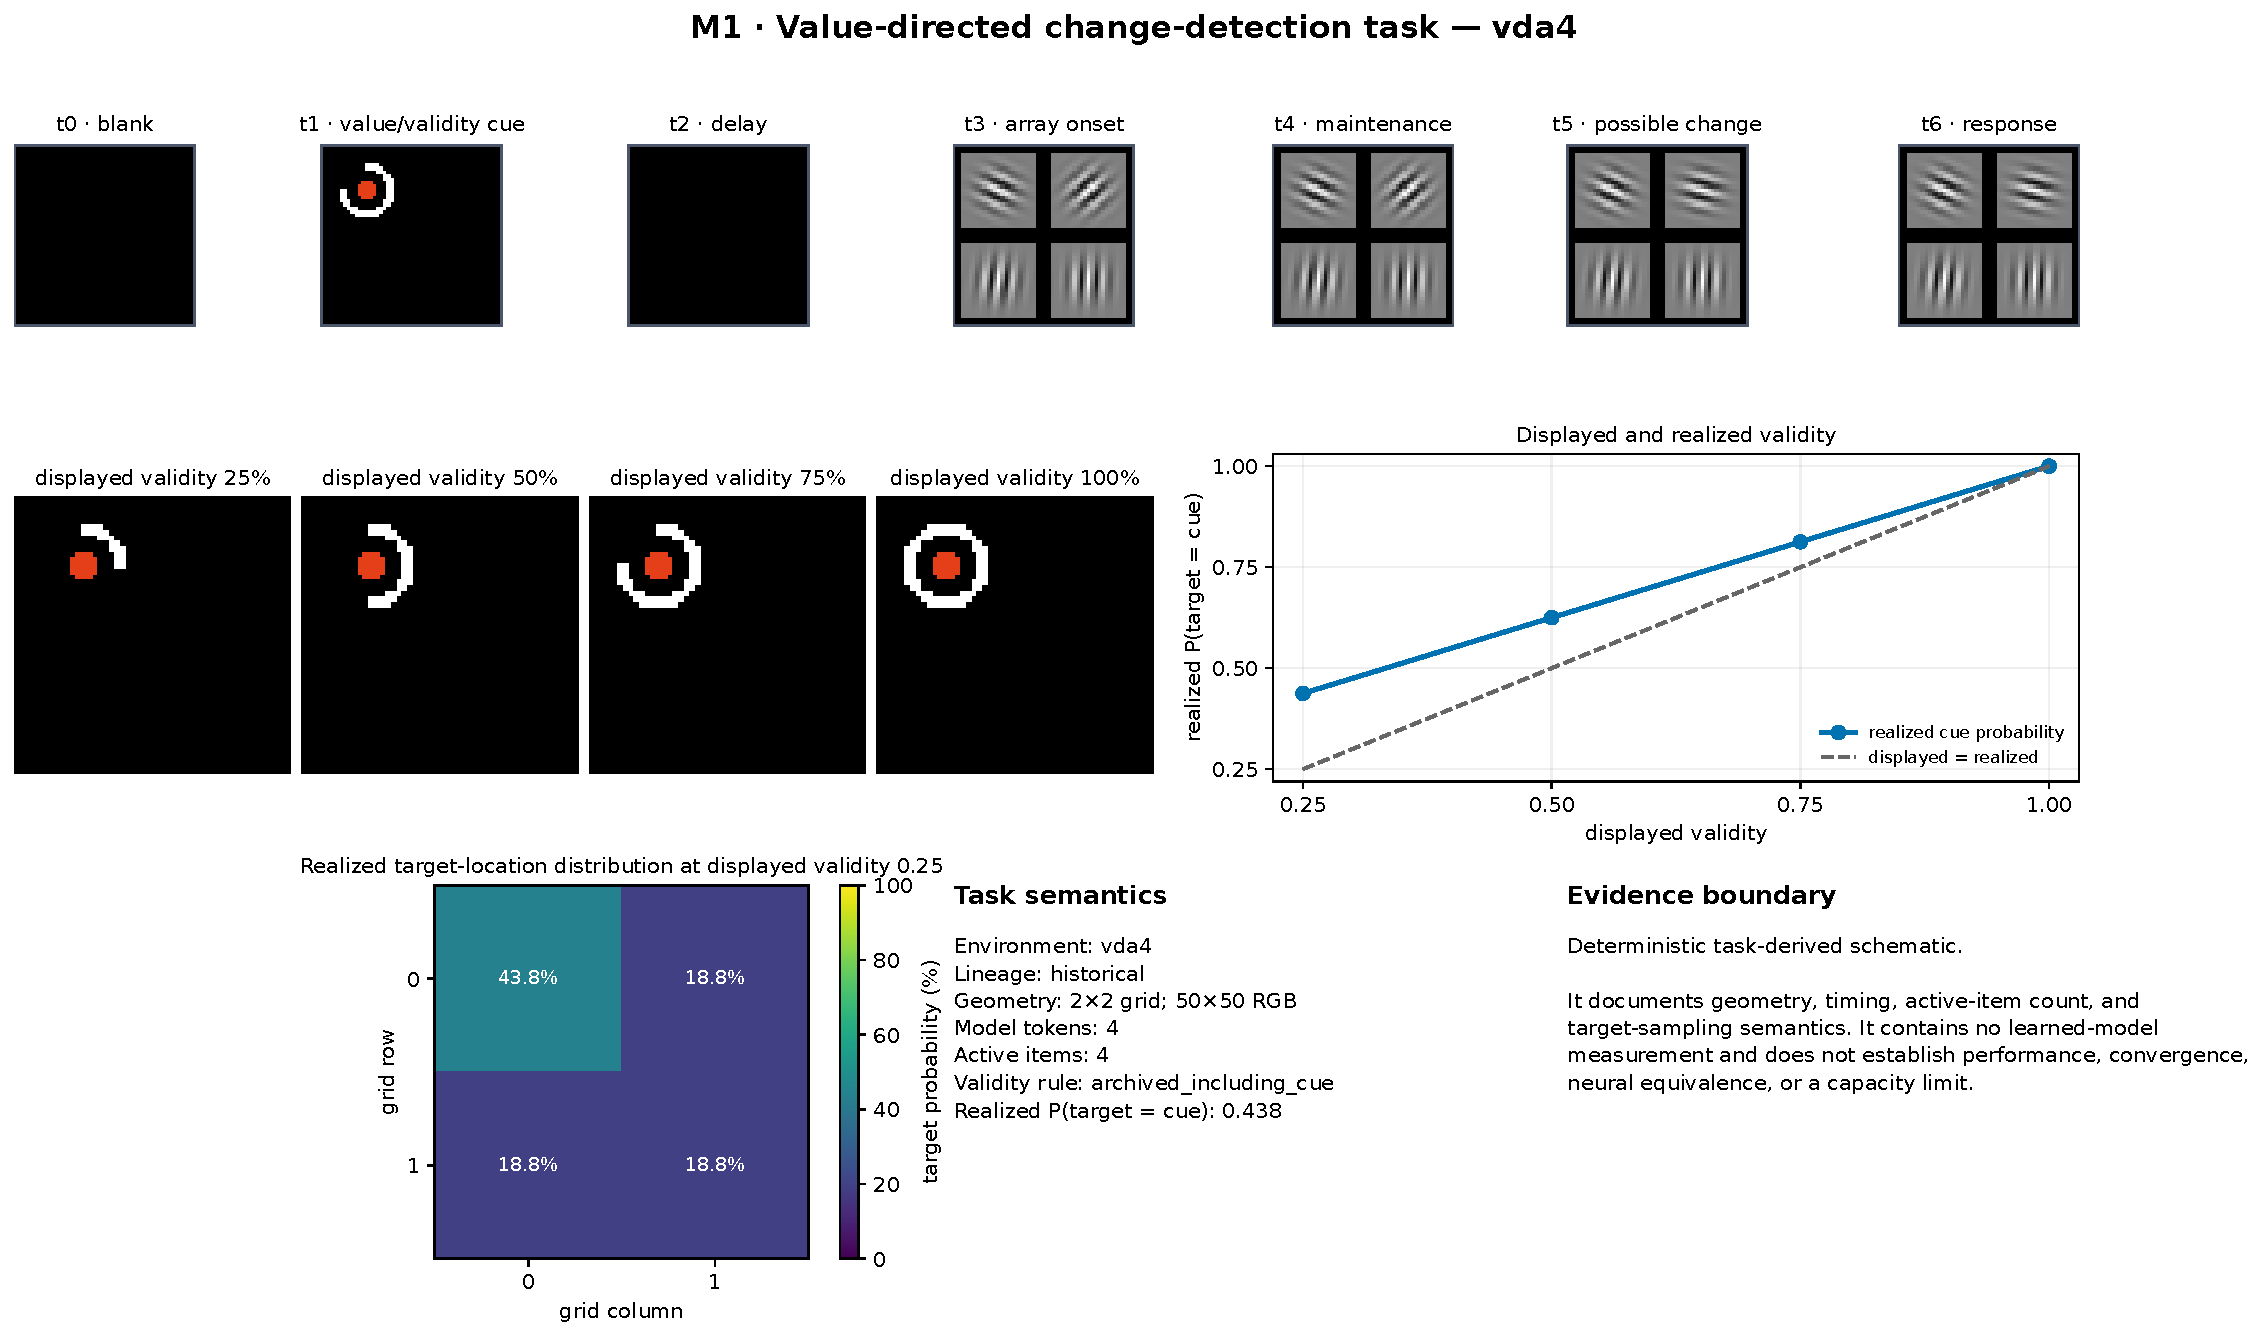
\includegraphics[width=0.47\linewidth]{m1_task_vda4.pdf}\hfill
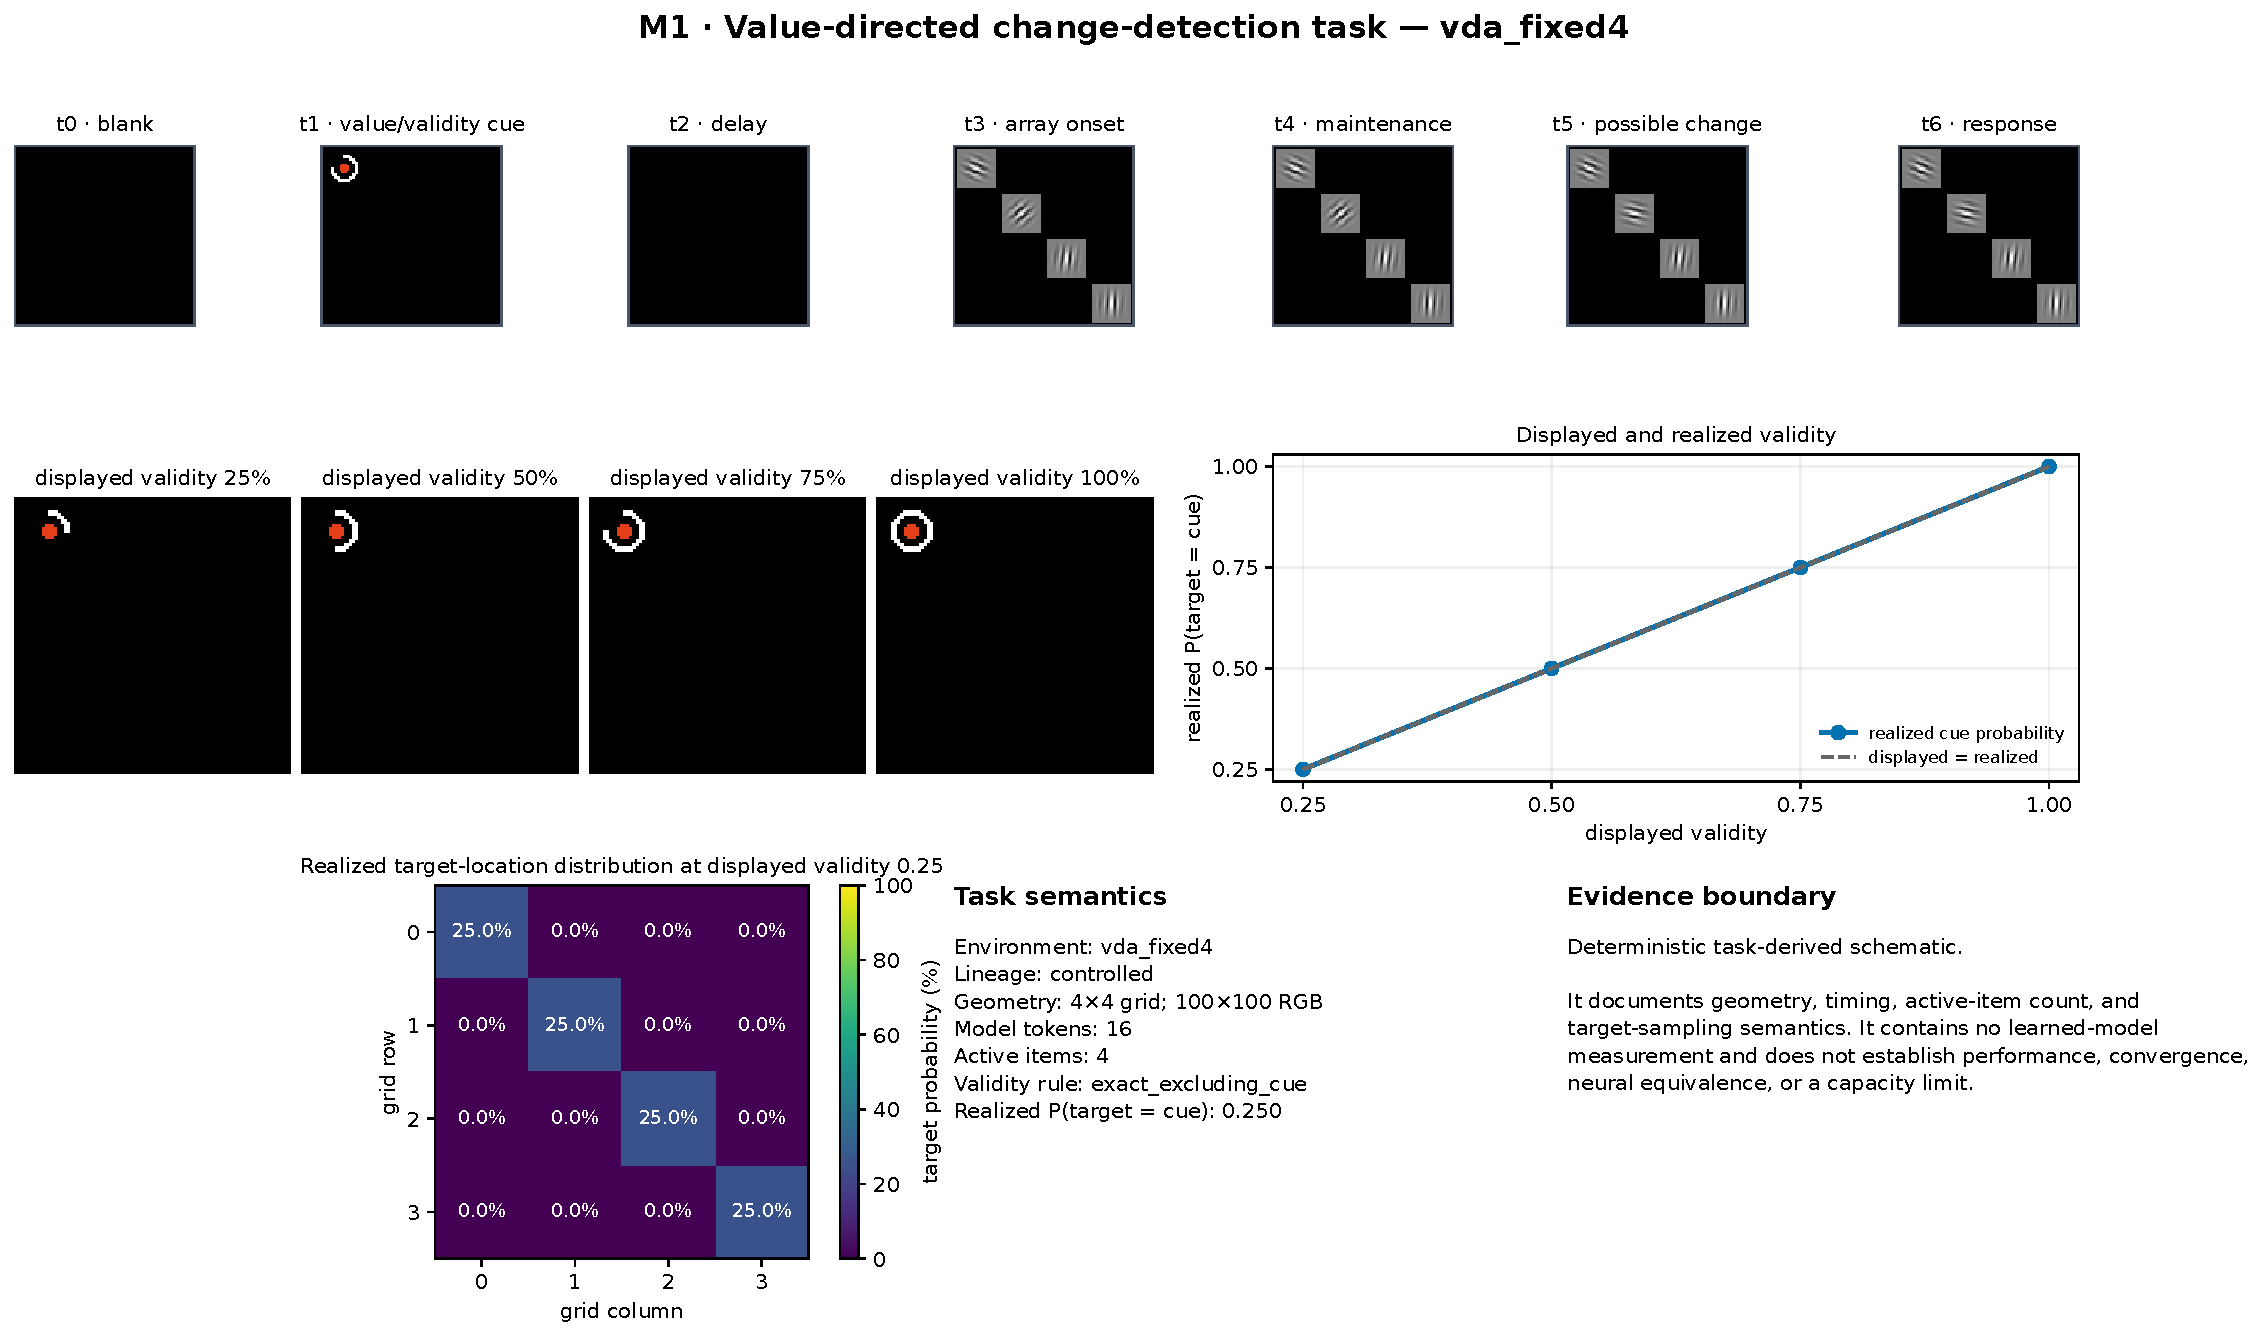
\includegraphics[width=0.47\linewidth]{m1_task_vda_fixed4.pdf}
\caption{Historical VDA4 (left) and controlled fixed-grid VDA4 (right). The visible task is similar, but the grid and cue-validity semantics differ. These are deterministic specifications, not behavioral evidence.}
\label{fig:ln-task}
\end{figure}

Current visual patches become spatial tokens. Memory-conditioned routing transforms them, a shared recurrent rule updates one hidden state per represented location, and actor/critic heads read the combined state. Affine feedback uses the previous hidden state to generate scale and shift before visual self-attention. Cross-attention uses current-image queries and a joint key/value block containing current-image tokens $X_t$ followed by previous recurrent hidden states $H_{t-1}$. These are different routing architectures, not two names for the same map.

\begin{figure}[H]
\centering
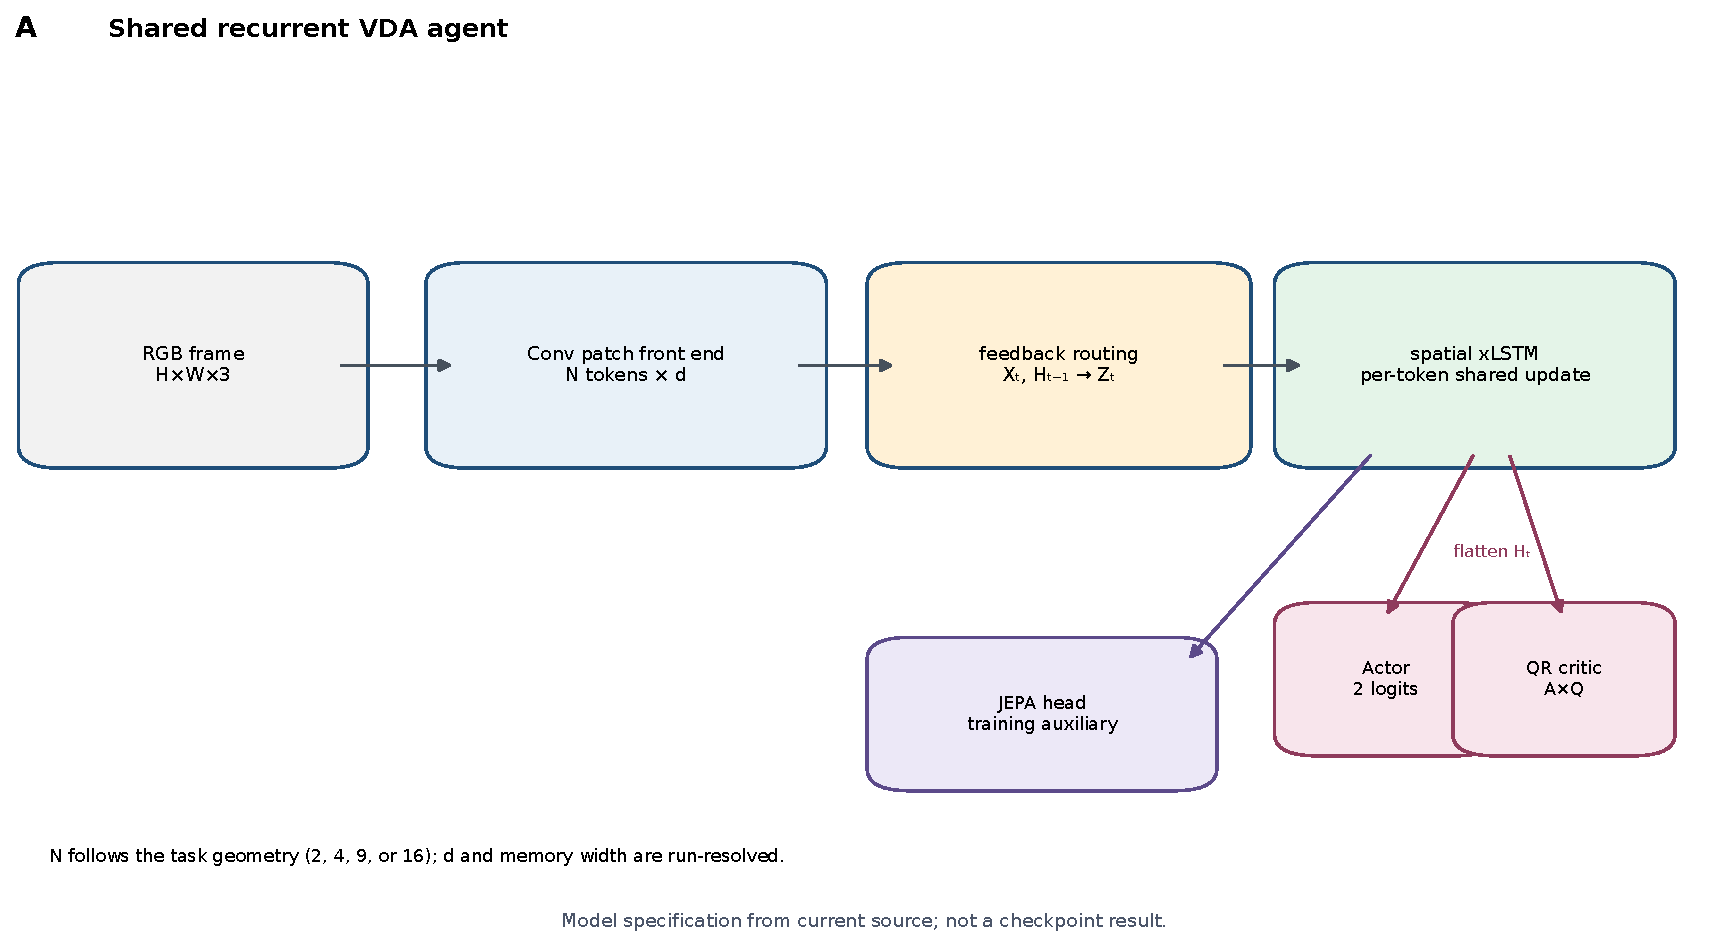
\includegraphics[width=0.92\linewidth]{m2_architecture_a.pdf}\\[4pt]
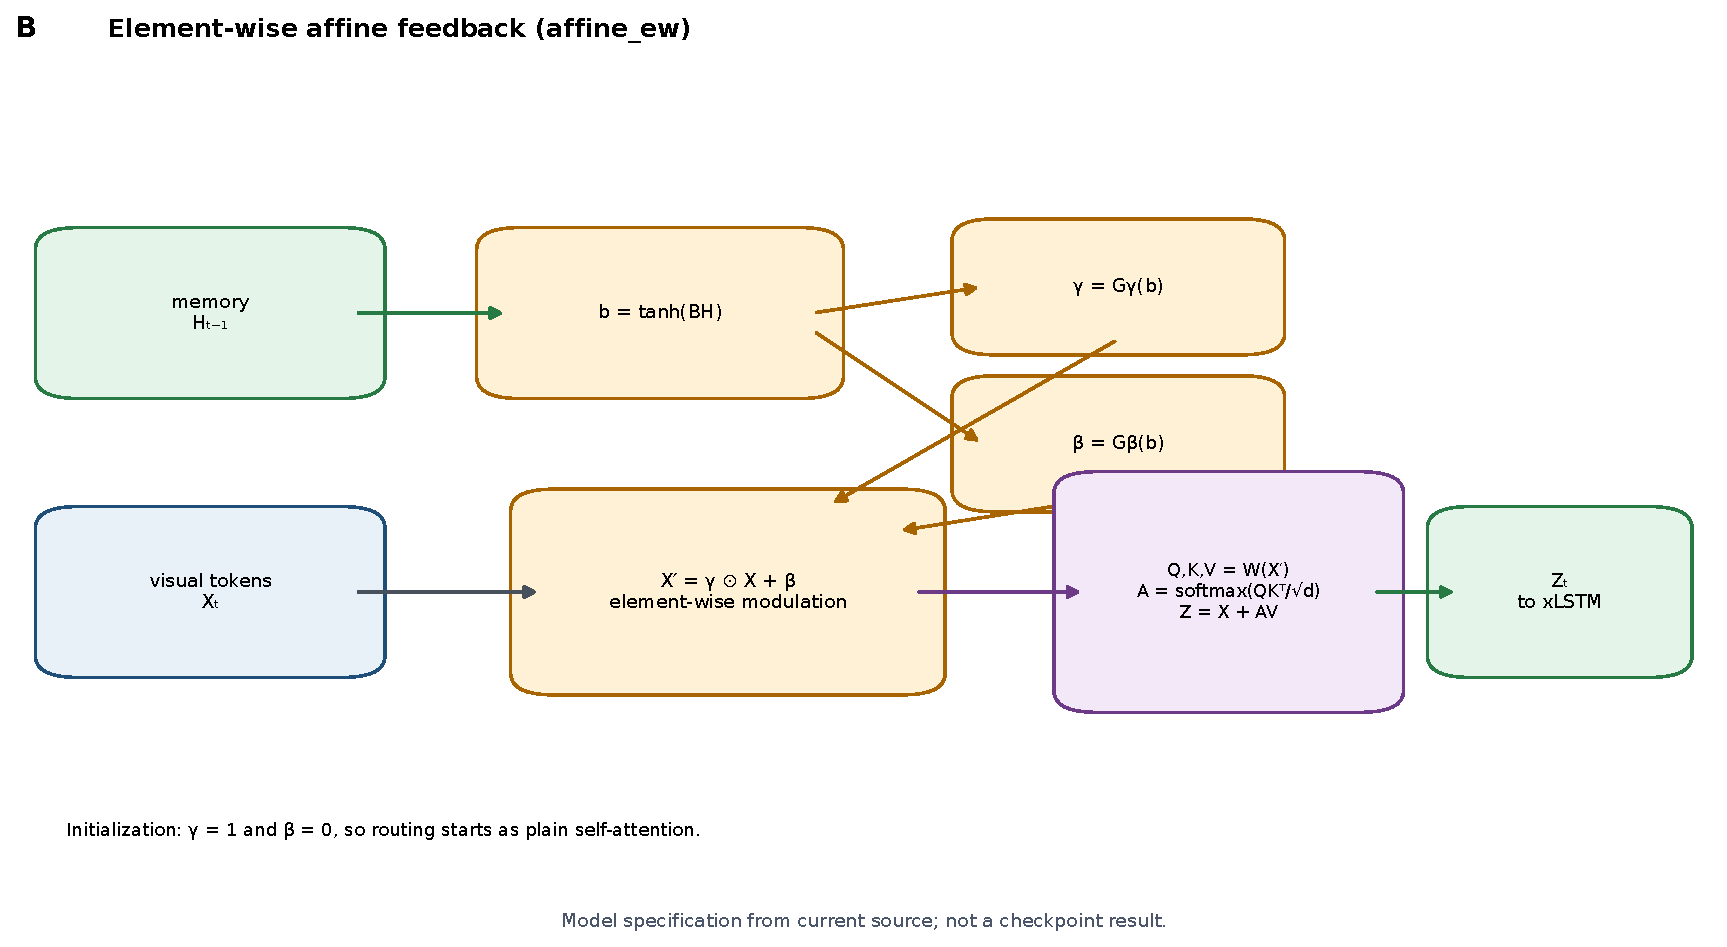
\includegraphics[width=0.43\linewidth]{m2_architecture_b.pdf}\hfill
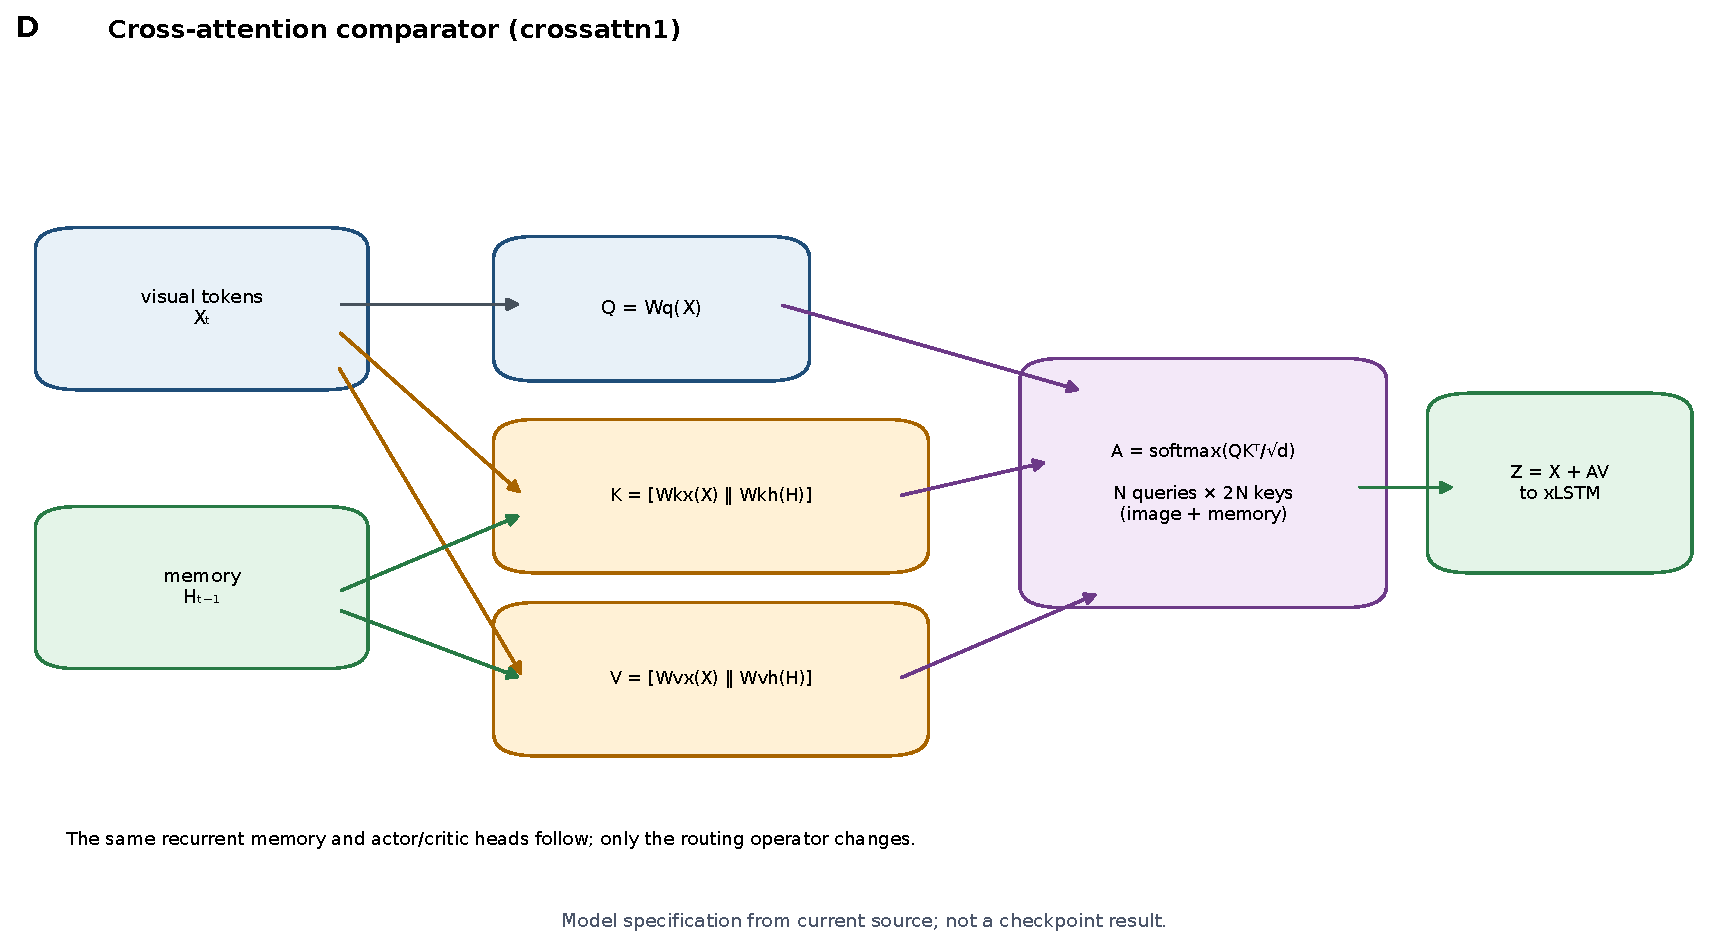
\includegraphics[width=0.43\linewidth]{m2_architecture_d.pdf}
\caption{Shared recurrent pipeline (top), affine feedback (bottom left), and cross-attention feedback (bottom right). In the affine model, $H_{t-1}$ modulates the current-image tokens before an $N\times N$ self-attention operation; there is no separate hidden-state-key map. In the cross-attention model, $N$ current-image queries attend jointly to $N$ keys projected from $X_t$ and $N$ keys projected from $H_{t-1}$ under one softmax.}
\label{fig:ln-architecture}
\end{figure}

\smallcapslabel{Terminology used in every attention figure.}
The notebook avoids the underspecified phrases ``input attention,'' ``memory attention,'' and ``cross-attention map'' unless the relevant tensor block is named. The following terms are architecture specific.

\begin{table}[H]
\centering\small
\begin{tabularx}{\linewidth}{@{}L{0.21\linewidth}L{0.31\linewidth}Y@{}}
\toprule
\smallcapslabel{Term} & \smallcapslabel{Exact quantity} & \smallcapslabel{Meaning and exclusion}\\
\midrule
Current-image-key routing (legacy label: visual-key) & $p^X_j=N^{-1}\sum_q A_{qj}$ in a cross-attention model & Query-averaged incoming mass to the key projected from $X_{t,j}$; this replaces the ambiguous phrase ``input attention.''\\
Previous-hidden-state-key routing (legacy label: memory-key) & $p^H_j=N^{-1}\sum_q A_{q,N+j}$ in a cross-attention model & Query-averaged incoming mass to the key projected from $H_{t-1,j}$; it is not attention occurring inside memory and is not an xLSTM cell-state or ``memory-slot'' map.\\
Cross-attention & Full routing matrix $A=[A^X\mid A^H]\in\mathrm{R}^{N\times2N}$ & $N$ current-image queries share one softmax over both key blocks. A source-specific map must say current-image-key or previous-hidden-state-key.\\
Affine self-attention & Self-attention after $X'_{t,j}=\gamma(H_{t-1,j})\odot X_{t,j}+\beta(H_{t-1,j})$ & A different routing family with $N$ current-image/self keys. The previous hidden state changes the image representation but is not a separately selectable key source.\\
Legacy paired-location sum (withdrawn) & $p^X_j+p^H_j$ & Combines two different key sources. It is not an attention source and is excluded from spatial maps and source-specific claims.\\
\bottomrule
\end{tabularx}
\caption{Architecture-grounded attention vocabulary. Routing family, key source, query reduction, spatial aggregation, and event frame are separate labels and must all be stated.}
\label{tab:ln-attention-terms}
\end{table}

\smallcapslabel{Frozen display rule for cross-attention.}
For attention tensor $A_{bqk}$, split current-image-key block $A^X$ and previous-hidden-state-key block $A^H$ before query reduction. Average down each key's query column to obtain $p^X$ and $p^H$, map those two vectors separately, and use one raw color scale with source share $w^X$ and $w^H$ printed. Do not sum the blocks into a spatial ``attention map.'' A cache that retains only the sum cannot support a source-resolved attention figure and must be excluded from attention claims.

\decisionbox{Green}{The architecture supports a precise, spatially registered intervention and a source-resolved analysis. Interpretability is designed in, but architecture alone is not attention, behavioral, or mechanism evidence.}

\section{Entry LN-02: Cued behavior and sensitivity}
\entrymeta{\statusmixed}{Held-out psychometrics and signal detection}{Does the model behave like a cued observer, and is the cueing effect sensitivity rather than response bias?}{Frozen checkpoint; held-out trial within checkpoint}

\smallcapslabel{Design.}
Checkpoint-recomputed psychometrics force the change to a fixed cued or opposite location while sweeping displayed cue proportion and orientation-change magnitude. Most points use 300 trials. Qualifying response probability counts only declarations at or after t5. No-change arms permit false-alarm, $d'$, and criterion estimates. Trial intervals describe one checkpoint; independent seeds are required for population inference.

\smallcapslabel{Result 1: the active-item pattern motivates the theory.}
In cross-attention, the fitted valid-minus-invalid threshold shift increases from $5.3^\circ$ at VDA4 to $10.9^\circ$ at VDA16; the response-probability gap near $18^\circ$ grows 0.27, 0.32, 0.44 over set sizes 4, 9, and 16. Affine grows and then plateaus/falls: threshold shifts $3.4^\circ$, $6.5^\circ$, $6.2^\circ$ and response gaps 0.19, 0.38, 0.32. VDA16 belongs to a different controlled lineage and is competence gated, so the open diamonds below are context, not a fitted continuation.

\begin{figure}[H]
\centering
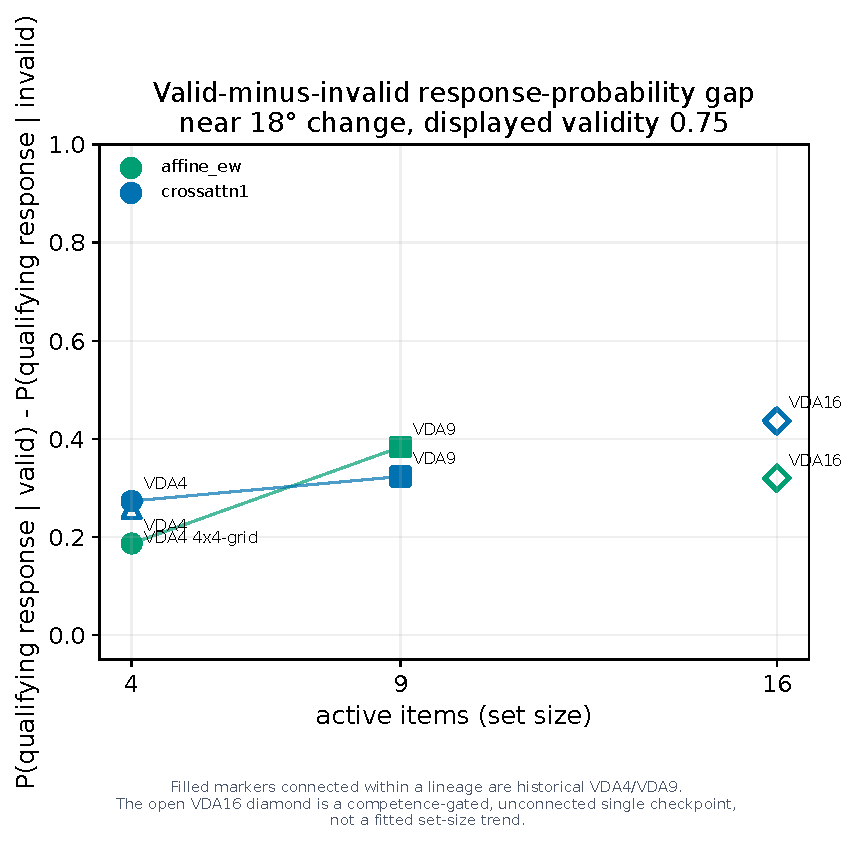
\includegraphics[width=0.64\linewidth]{psychometric_fit_setsize_summary.pdf}
\caption{Cueing-effect magnitude versus active-item set size. The cross-attention sequence is motivating evidence; the affine sequence prevents a universal capacity-law claim.}
\label{fig:ln-setsize-summary}
\end{figure}

\smallcapslabel{Result 2: VDA16 cueing includes discriminability.}
At displayed validity 0.75 and an $18^\circ$ change, cross-attention $d'$ rises from 0.56 forced-invalid to 1.80 valid while criterion falls from 1.27 to 0.66. Affine $d'$ rises from 2.01 to 2.97 while criterion falls from 0.93 to 0.45. Both routing families therefore show a sensitivity gap, not only a more liberal declaration policy; cross-attention's proportional sensitivity change is larger.

\begin{figure}[H]
\centering
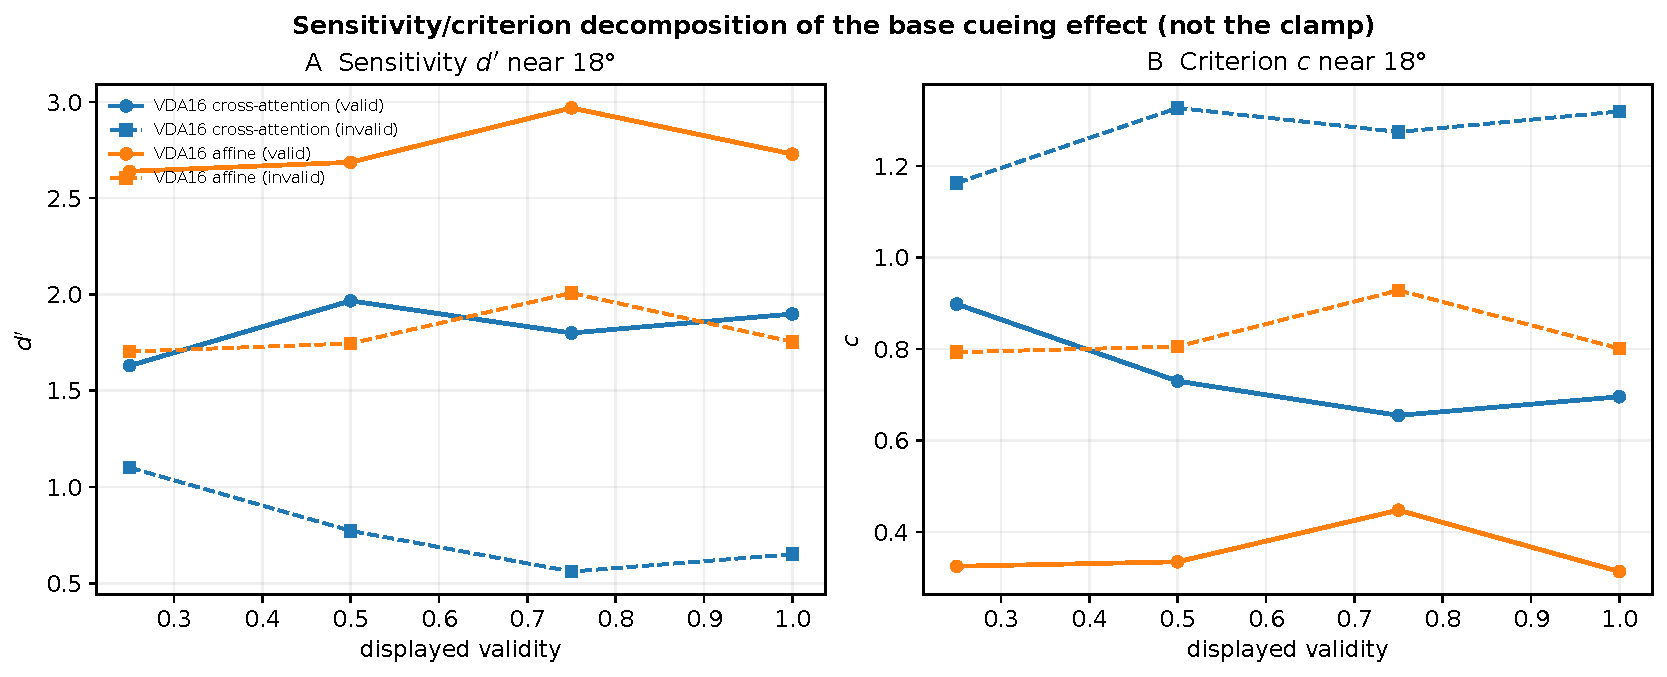
\includegraphics[width=0.86\linewidth]{baseline_sdt_decomposition.pdf}
\caption{Unmanipulated VDA16 sensitivity and criterion. Solid lines are valid trials; dashed lines are forced-invalid. This is the appropriate behavioral bridge to an attention mechanism claim.}
\label{fig:ln-baseline-sdt}
\end{figure}

\smallcapslabel{Interpretation boundary.}
The cross-attention set-size pattern is compatible with greater selection pressure when more objects compete, but VDA4/VDA9 and VDA16 differ in geometry, task lineage, training trajectory, and checkpoint competence. The $d'$ decomposition currently covers the two VDA16 checkpoints, not the whole set-size ladder.

\decisionbox{Amber}{Cued behavior is real and sensitivity relevant at VDA16. Growth with set size remains a routing-family-specific, single-checkpoint descriptive pattern—not yet a controlled scaling result.}

\section{Entry LN-03: Current-image-key and previous-hidden-state-key routing over time}
\entrymeta{\statusmixed}{Held-out routing description}{Do current-image-key and previous-hidden-state-key routing align with the cue and with a later physical change?}{Frozen checkpoint; trial; named logical frame}

\smallcapslabel{Design.}
No-change trials isolate cue maintenance: the cue is fixed, nothing physically changes, and t5 is only the nominal change opportunity. A separate VDA16 common-random-number bank contains actual cued or forced-invalid changes. Primary cross-attention maps are split into current-image-key and previous-hidden-state-key blocks. The older paired VDA16 cache retained only their co-located sum; that cache is now excluded from attention visualization. Map evidence is event aligned but correlational.

\smallcapslabel{Result 1: the two sources have different temporal profiles.}
In VDA4 cross-attention, current-image-key and previous-hidden-state-key maps do not justify a single fused ``cross-attention map.'' Previous-hidden-state keys often carry most of the joint-softmax mass, while current-image-key share and localization change with cue validity and frame. The panels below repeat the established display convention separately for each source rather than collapsing co-located keys.

\begin{figure}[H]
\centering
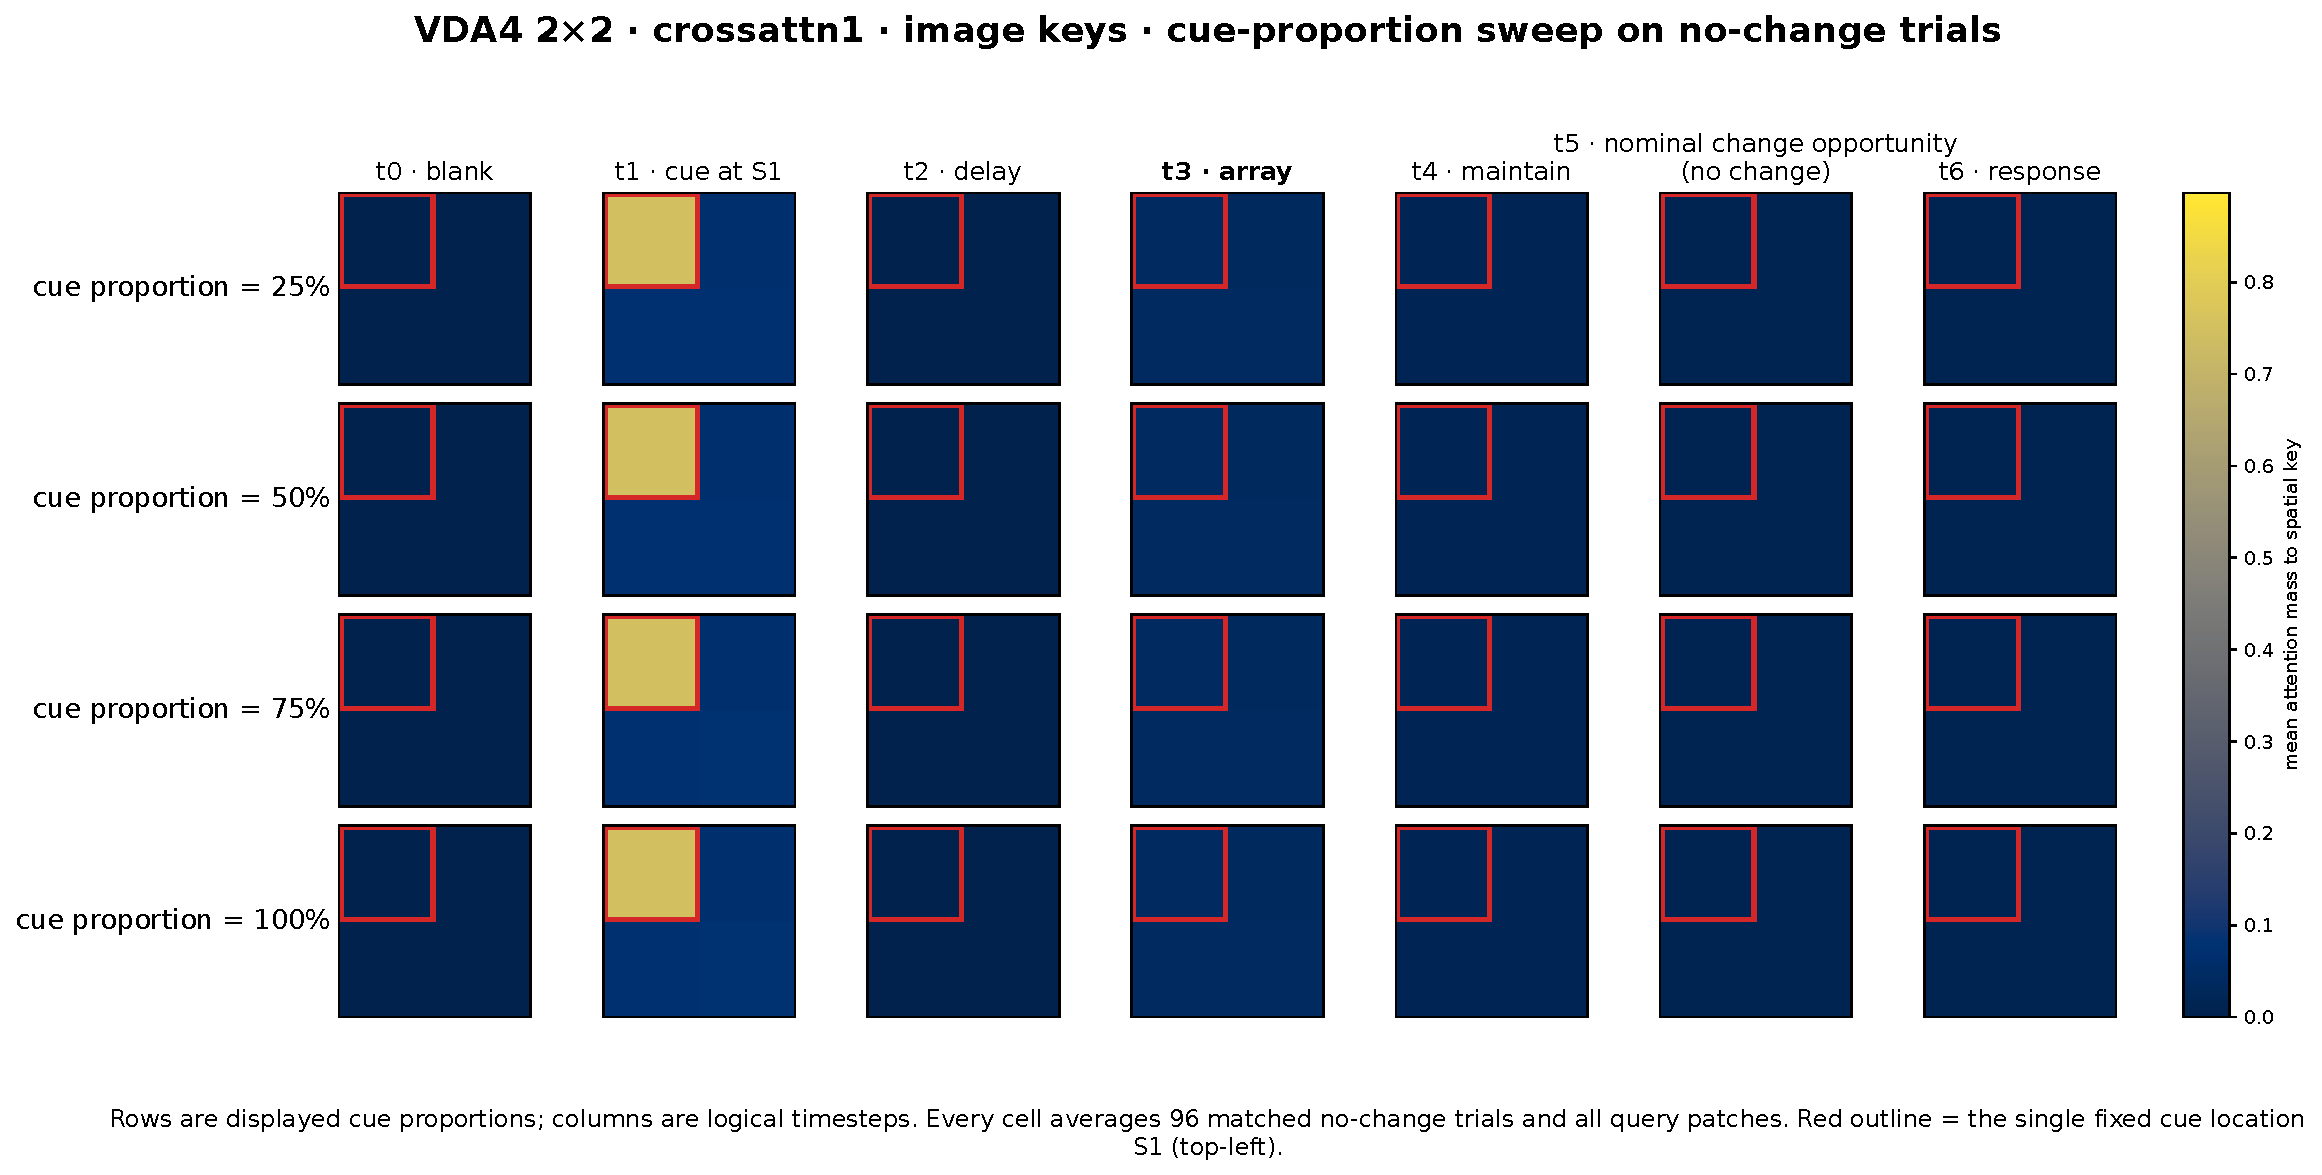
\includegraphics[width=0.48\linewidth]{first_wave_attention_vda4_crossattn1_image_keys.pdf}\hfill
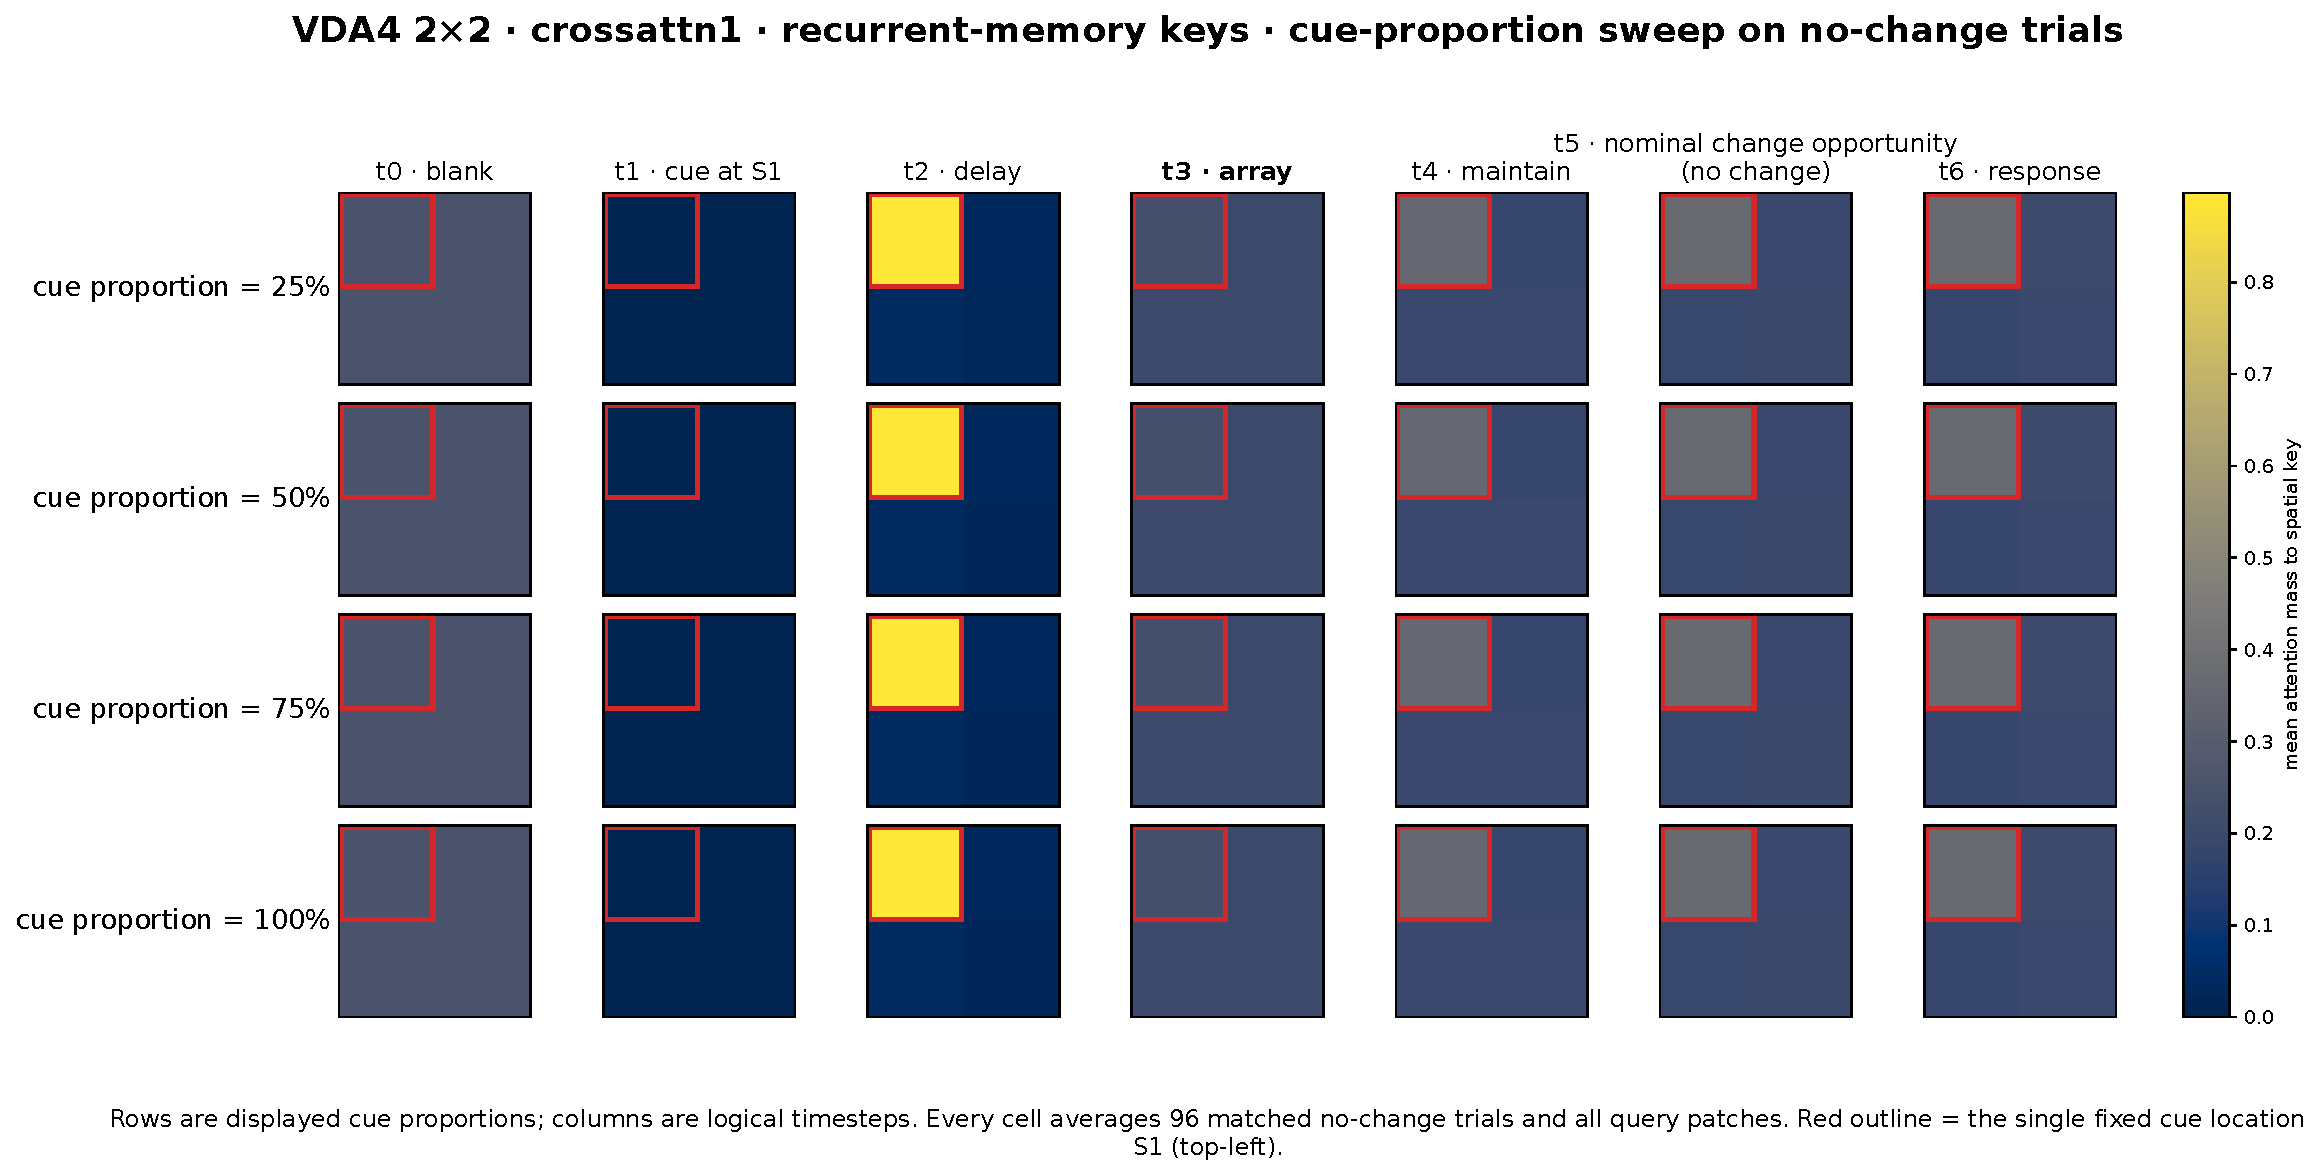
\includegraphics[width=0.48\linewidth]{first_wave_attention_vda4_crossattn1_recurrent_memory_keys.pdf}
\caption{VDA4 cross-attention no-change routing. Left: query-averaged incoming mass $p^X$ to keys projected from current-image tokens $X_t$. Right: query-averaged incoming mass $p^H$ to keys projected from the previous recurrent hidden output $H_{t-1}$. The embedded legacy headings ``image keys'' and ``recurrent-memory keys'' refer to these two blocks. Neither block is renormalized within source; both preserve their absolute share under the same joint $2N$-key softmax and use one common raw scale. No affine checkpoint appears. These maps describe allocation, not representation quality or causal use.}
\label{fig:ln-vda4-sources}
\end{figure}

The same separation at VDA16 shows current-image-key changes near cue onset and strong previous-hidden-state-key allocation after the cue and through the blank delay. Persistent delay-period routing is compatible with memory-supported priority maintenance, but a delay disruption is needed before calling it rehearsal.

\begin{figure}[H]
\centering

\includegraphics[width=0.48\linewidth]{first_wave_attention_vda16_crossattn1_image_keys.pdf}\hfill

\includegraphics[width=0.48\linewidth]{first_wave_attention_vda16_crossattn1_recurrent_memory_keys.pdf}
\caption{VDA16 cross-attention no-change routing. Left is $p^X$ to current-image keys; right is $p^H$ to previous-hidden-state keys. The two blocks preserve absolute mass under one joint $2N$-key softmax and use one common raw scale; they are never added. The embedded panel headings are legacy aliases. No affine checkpoint appears.}
\label{fig:ln-vda16-sources}
\end{figure}

\smallcapslabel{Audit correction: the legacy paired attention visualization is withdrawn.}
The paired evaluator saved only $p^X_j+p^H_j$, after which it discarded the raw current-image-key block $A^X$ and previous-hidden-state-key block $A^H$. Summing those sources does not produce an interpretable attention map. The earlier panels are therefore removed rather than relabeled. Their duplicated t4 appearance was expected because the common-random-number branches were physically identical before the t5 manipulation, but that fact does not rescue the invalid source aggregation. Branch-specific source maps at t4 and t5 require a fresh checkpoint evaluation that preserves $A^X$ and $A^H$ separately. No branch-specific attention conclusion is drawn from this cache.

The held-out behavioral arrays in the same cache remain interpretable because they do not depend on the withdrawn attention reduction. Figure~\ref{fig:ln-vda16-paired-behavior} therefore retains response probability and discrete response frame only.

\begin{figure}[H]
\centering
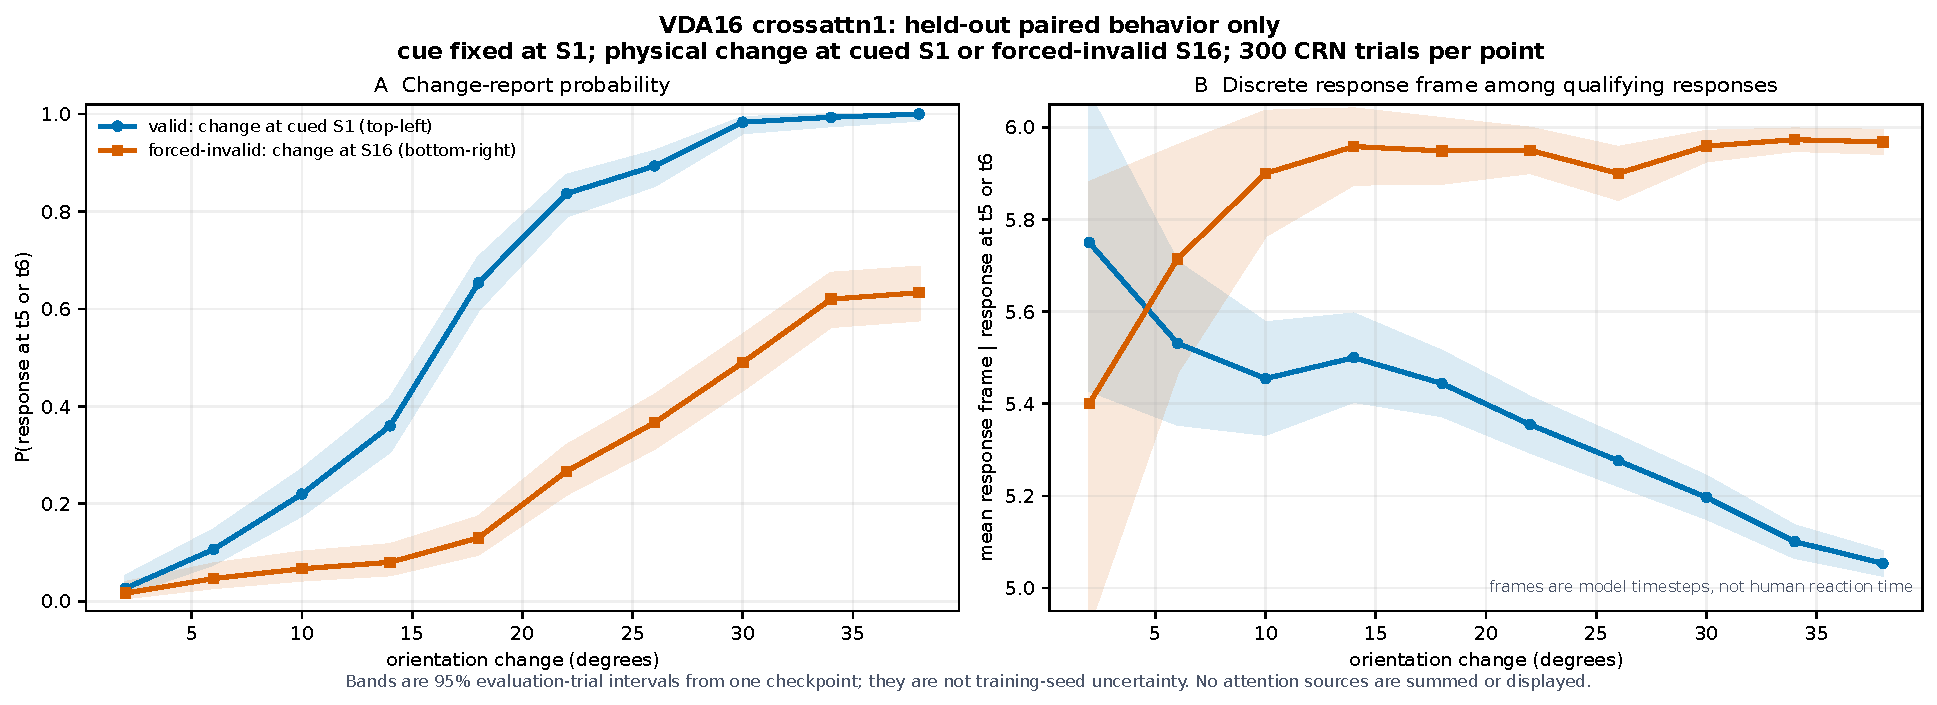
\includegraphics[width=0.92\linewidth]{vda16_cued_vs_opposite_behavior_only.pdf}
\caption{VDA16 \texttt{crossattn1} held-out paired behavior only. The cue is fixed at S1; the physical change occurs either at valid S1 or forced-invalid S16 over 300 matched trials per magnitude. Panel A reports qualifying response probability. Panel B reports the model's discrete response frame conditional on responding; it is not human reaction time. Bands are finite evaluation-trial intervals from one checkpoint, not training-seed uncertainty or paired-difference intervals. No attention sources are summed or displayed, and this change-present bank cannot by itself estimate $d'$ or criterion.}
\label{fig:ln-vda16-paired-behavior}
\end{figure}

\smallcapslabel{Temporal warning.}
In the fixed-four-item grid battery, forced-invalid true-change-minus-cue routing is negative at frame 5 and positive at frame 6. The reversal is nearly all previous-hidden-state-key routing. Frame 6 is an evaluator-continued, post-change/open-loop state and cannot be averaged with frame 5 without changing the estimand.

\decisionbox{Amber}{The source-separated no-change maps track the cue over time. Branch-specific t5 routing remains unmeasured until the paired evaluator is rerun with both key blocks preserved. The retained maps are correlational; the causal test must target the same location and frame.}

\section{Entry LN-04: Spatially specific causal rescue}
\entrymeta{\statuslocal}{Producer-bound held-out causal intervention}{Is routing at the true change location necessary and sufficient for detection at this checkpoint?}{One competence-gated trained checkpoint; 300 CRN trials per condition}

\smallcapslabel{Frozen test.}
On forced-invalid VDA16 trials with a $30^\circ$ change, the identical graded pre-softmax bias is applied from t5 onward at one of three roles: true change location, cued-but-wrong location, or neutral location. The test requires both directions—suppression and boost—and location controls. Signal detection reports $d'$ and criterion beside response rate.

\smallcapslabel{Central result.}
At unbiased invalid baseline, qualifying response is 51\% and $d'=1.91$. Suppressing the true change location reduces response to 7\% and $d'$ to 0.38. Boosting it raises response to 95\% and $d'$ to 3.33, closing 92\% of the gap to the independently measured 98\% valid-cue ceiling. Among trials that respond, the discrete response frame remains about 5.5--6.0: the intervention changes whether the model detects the change more than when it declares after detection.

The same operation at controls does not rescue behavior. Suppressing the cued-but-wrong location changes response from 51\% to 54\%; boosting it lowers response to 42\% and raises false alarms from 3\% to 25\%. Suppressing neutral is similarly inert (53\%); boosting neutral lowers response to 9\%. Boosting either control competes away mass at the true target.

\begin{figure}[H]
\centering
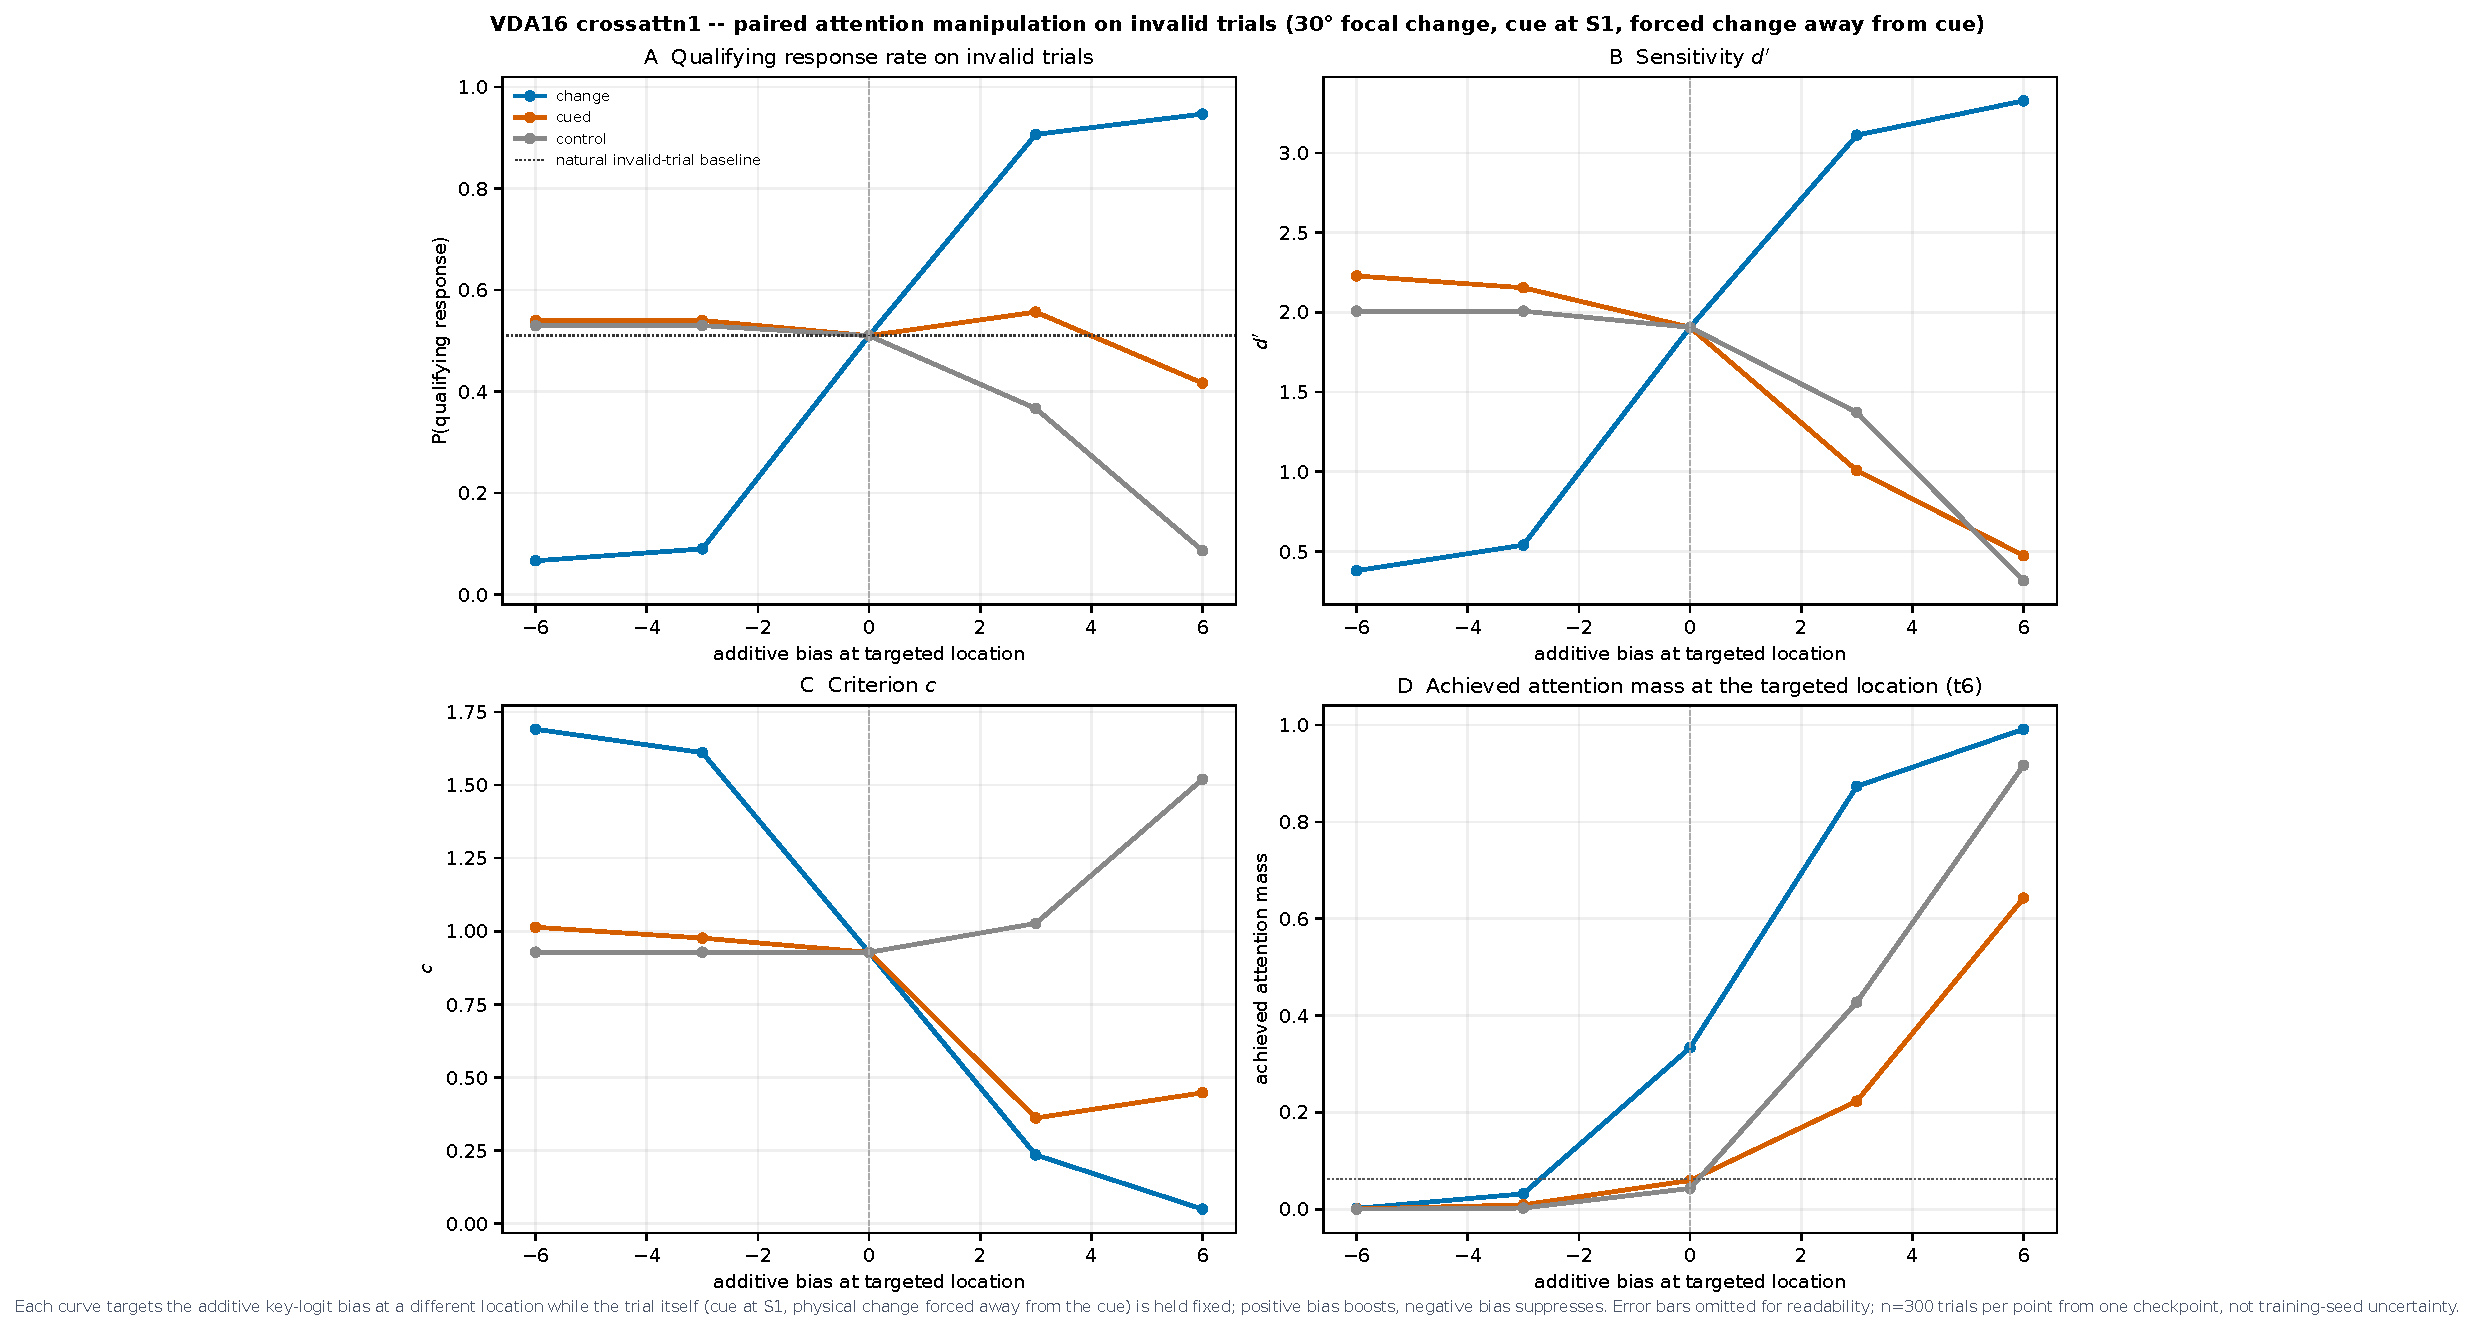
\includegraphics[width=0.92\linewidth]{vda16_change_location_intervention_summary.pdf}
\caption{The central VDA result: only a bias targeted at the true change location produces the predicted bidirectional rescue. Panels jointly report response, $d'$, criterion, and achieved attention.}
\label{fig:ln-central-causal}
\end{figure}
\whyitmatters{A cue-linked map could have been epiphenomenal. The true/wrong/neutral double dissociation shows that spatially matched routing is behaviorally used inside this checkpoint.}

\begin{figure}[H]
\centering
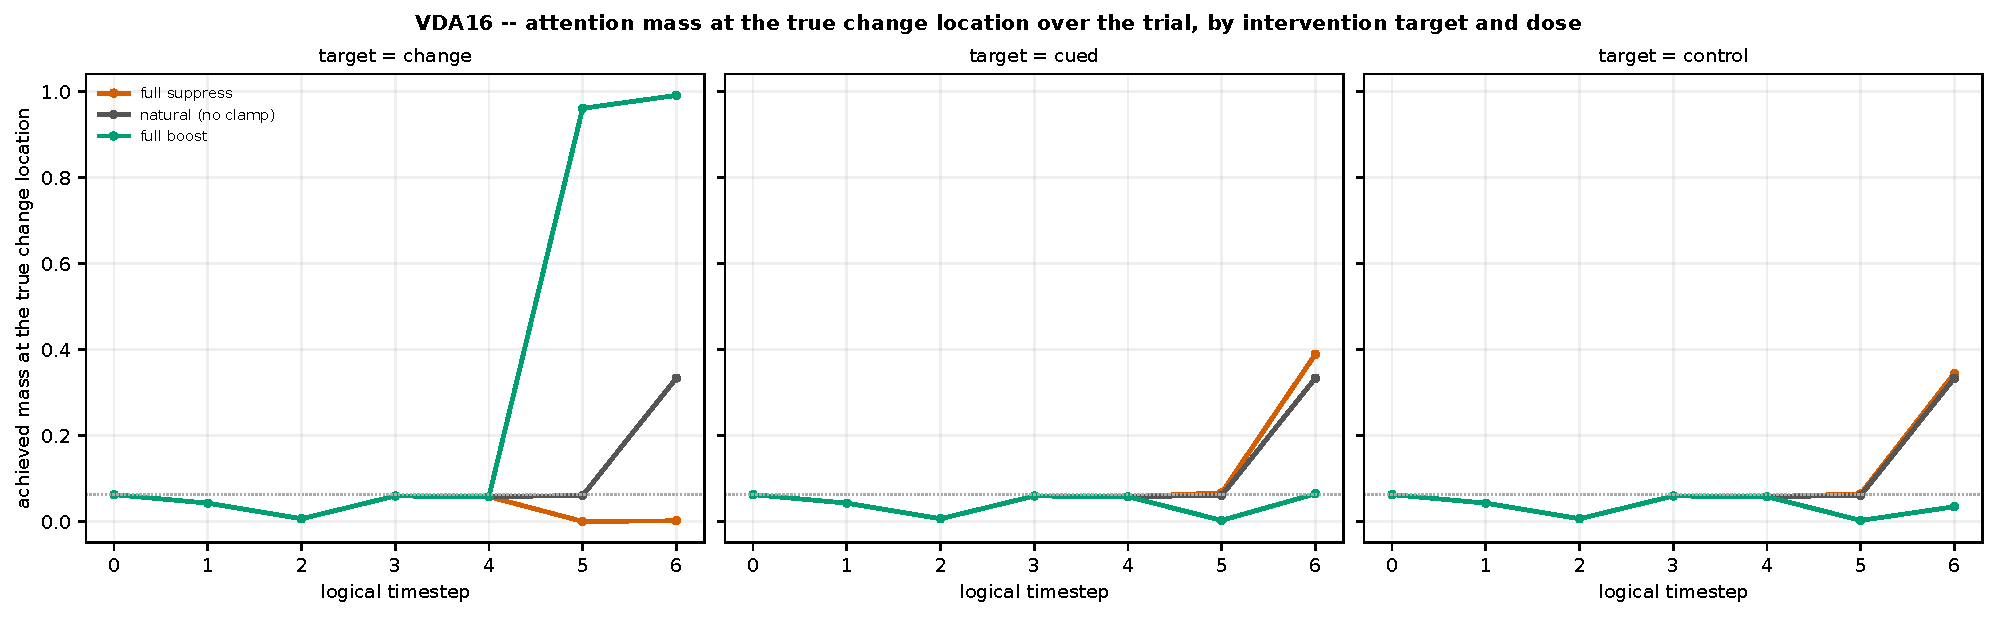
\includegraphics[width=0.74\linewidth]{vda16_change_location_attention_trajectory.pdf}
\caption{Achieved attention at the true change location across the trial. Direct true-location targeting raises its mass; forcing either control location lowers it competitively.}
\label{fig:ln-central-trajectory}
\end{figure}

\smallcapslabel{Bounded VDA4 scale-down.}
The same design in a fresh VDA4 cross-attention checkpoint preserves the ordering but not the full curve shape. The invalid baseline is 42\% ($d'=1.32$), true-location suppression reduces response to 27\% ($d'=0.90$), and boost raises it to 59\% ($d'=1.83$). Suppressing the cued-wrong location now helps (42\% to 51\%), consistent with possible four-location softmax spillover but not isolating that mechanism. Neutral produces the smallest swing.

\begin{figure}[H]
\centering
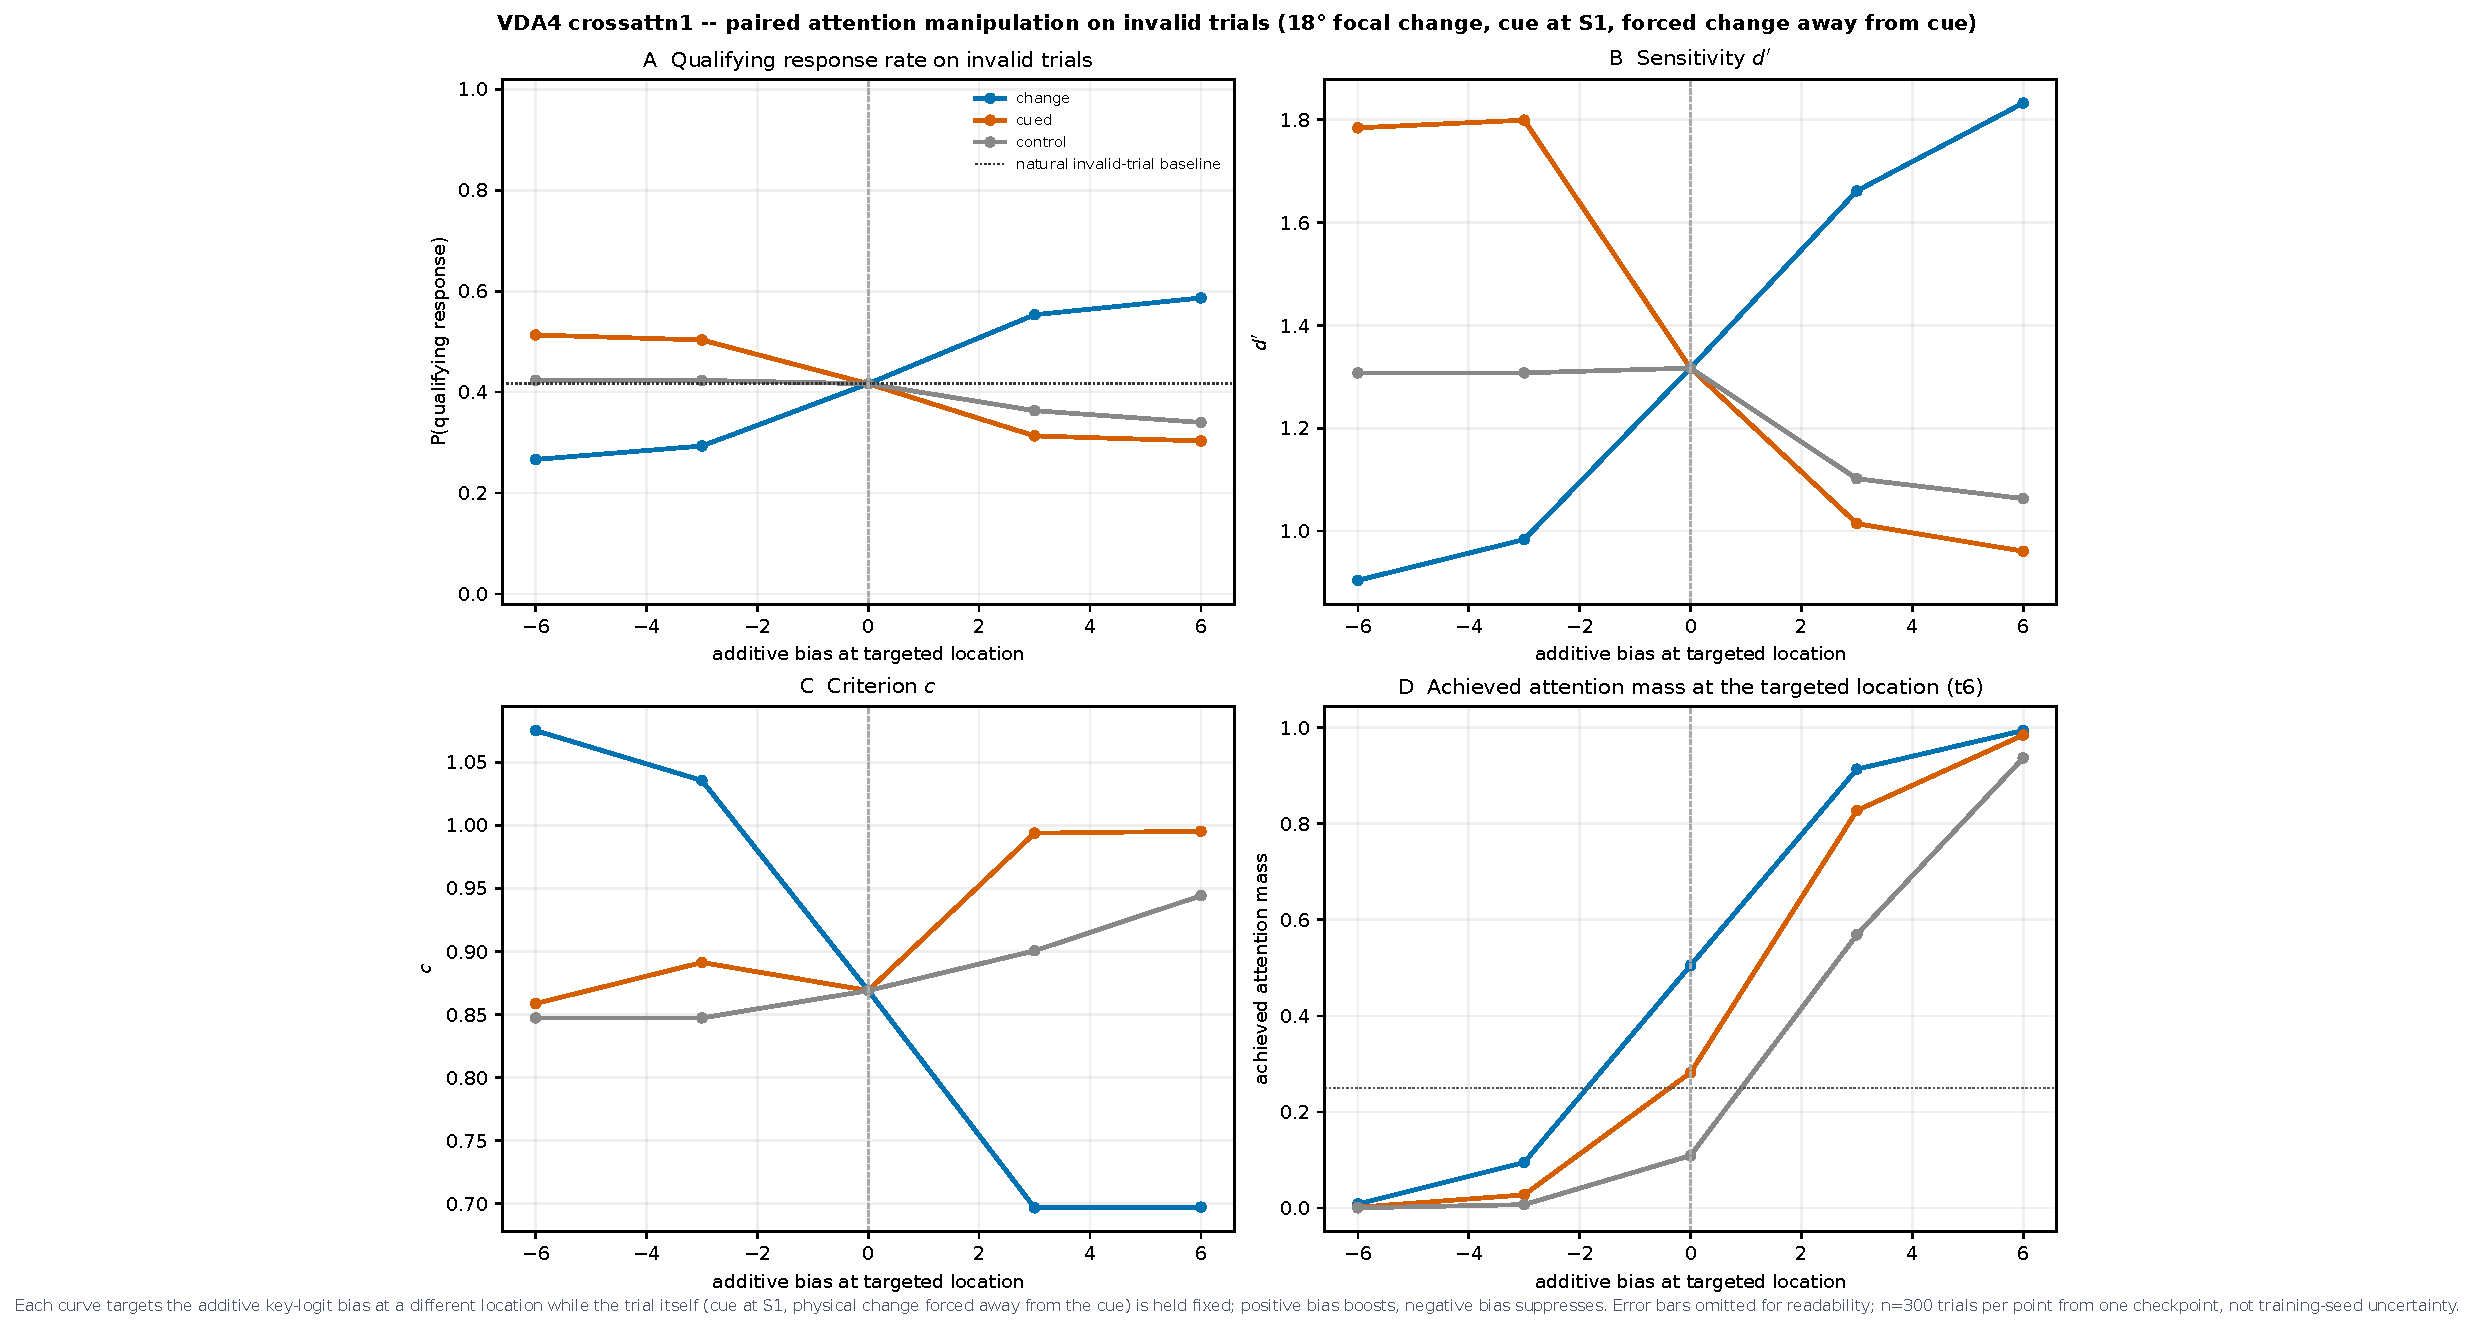
\includegraphics[width=0.86\linewidth]{vda4_change_location_intervention_summary.pdf}
\caption{VDA4 scale-down. True-location targeting remains the largest and most orderly effect, but control behavior differs from VDA16.}
\label{fig:ln-vda4-causal}
\end{figure}

\warningbox{The VDA16 and VDA4 cross-attention bundles are producer-bound and lack an independent semantic recomputation. They are single competent seed-0 checkpoints. The VDA4 checkpoint also used a newer documented PyTorch/CUDA stack. These interventions establish checkpoint-local routing dependence, not seed-general sufficiency or biological equivalence.}

\decisionbox{Green}{Spatially targeted routing causally controls detection at the evaluated cross-attention checkpoints, most strongly at VDA16. This is the best current support for the functional account, but it does not yet show that the intervention improves target representation or actor evidence.}

\section{Entry LN-05: The fixed-set-size discretization test}
\entrymeta{\statusnot}{Independently checked fixed-checkpoint held-out battery}{Does finer native patching increase cue dependence and causal routing leverage with four active items fixed?}{Six seed-0 checkpoints; limited two-seed cross-attention endpoints}

\smallcapslabel{Prediction.}
Increasing the native grid from $2\times2$ to $4\times4$ to $10\times10$ increases patch-level alternatives around the same four objects. The simple prediction was monotonic: stronger uniform-normalized target allocation, larger sensitivity-corrected cueing, and larger spatially specific intervention effects at larger $N$.

\smallcapslabel{Design.}
The $2\times3$ battery crosses 4/16/100 tokens with cross-attention/affine routing. All seed-0 checkpoints use $d_\mathrm{mem}=128$, memory decay 1, the same curriculum and evaluator, and terminal iteration 19,999. Held-out counts are 300 psychometric trials per condition, 128 event trials per condition, and 250 intervention trials per condition. Cross-attention endpoints at 4 and 100 tokens add seed 1.

\smallcapslabel{Behavioral result.}
The 100\%-displayed invalid-minus-valid threshold costs across 4/16/100 tokens are $7.16^\circ$, $5.66^\circ$, $6.18^\circ$ for cross-attention and $2.63^\circ$, $2.60^\circ$, $4.24^\circ$ for affine. Normalized valid-minus-invalid response-gap AUC is 0.219, 0.170, 0.197 for cross-attention and 0.085, 0.079, 0.122 for affine. Invalid response at the easy $30^\circ$ anchor is 0.947--1.000 in every cell, leaving little mechanistic leverage.

\begin{figure}[H]
\centering

\includegraphics[width=0.91\linewidth]{vda4_spatial_scaling_seed0_summary.pdf}
\caption{Fixed-four-item native-grid battery. The behavioral, temporally averaged attention, and routing-disable panels reveal routing-family heterogeneity rather than one monotonic token-count law.}
\label{fig:ln-grid-summary}
\end{figure}

\smallcapslabel{Source-resolved result.}
For cross-attention seed 0, current-image-key source share over 4/16/100 tokens is 0.105, 0.060, 0.346; previous-hidden-state keys receive the complement. Current-image-key target-quadrant mass conditional on source is 0.242, 0.263, 0.247; the corresponding previous-hidden-state-key values are 0.533, 0.467, 0.301. Target maximum relative to a globally uniform key is 0.21, 0.24, 1.28 for current-image keys and 3.84, 5.88, 3.39 for previous-hidden-state keys. Affine valid-target total is 0.778, 0.928, 0.724 while its peak-quadrant share is 0.778, 0.944, 0.935. Different measures therefore answer different questions and do not converge on monotonic extremity.

\begin{figure}[H]
\centering

\includegraphics[width=0.96\linewidth]{attention_crossattn_source_metrics_seed0.pdf}
\caption{Current-image-key and previous-hidden-state-key sources remain separate. Source share, equal-area target total, raw maximum, uniform-normalized maximum, conditional target total, and peak-quadrant share are distinct estimands.}
\label{fig:ln-source-metrics}
\end{figure}

\begin{figure}[H]
\centering

\includegraphics[width=0.94\linewidth]{attention_crossattn_source_common_2x2_seed0.pdf}
\caption{Source-specific common-physical-grid totals and maxima. Rows identify native grid and key source; columns separate valid/invalid and total/maximum. Current-image-key and previous-hidden-state-key maps share scales and are never collapsed before the maximum.}
\label{fig:ln-source-common}
\end{figure}

\smallcapslabel{Timing result.}
On forced-invalid cross-attention trials, true-change-minus-cue co-located mass at frame 5 is $-0.309$, $-0.260$, $-0.047$ over 4/16/100 tokens, then reverses at frame 6 to 0.752, 0.249, 0.038. Memory accounts for nearly the entire reversal; all visual contrasts lie between $-0.0024$ and $+0.0011$. A frame-5--6 average obscures this processing sequence.

\smallcapslabel{Replication result.}
The 4-to-100-token direction reverses over cross-attention seeds. Memory-conditional valid-target total falls 0.533 to 0.301 in seed 0 but rises 0.291 to 0.549 in seed 1. Threshold cost changes by $-0.98^\circ$ in seed 0 and $+2.50^\circ$ in seed 1; response-gap AUC changes by $-0.022$ and $+0.076$; response-frame cost changes by $+0.050$ and $-0.030$. Seed-1 100-token behavior is saturated across routing modes.

\smallcapslabel{Causal dependence.}
Routing disable lowers invalid-response probability by 12.4, 8.0, 1.2 points for cross-attention and 38.4, 98.0, 99.2 points for affine. The operations are architecture specific—cross-attention retains a residual visual path—so these are not cross-family calibrated doses. Parameter count also co-varies with grid (approximately 2.2M, 3.0M, 8.7M).

\decisionbox{Red}{The simple monotonic discretization prediction is not supported. Native grid changes routing cardinality, spatial support, readout size, and parameters together; results depend on family, source, metric, frame, and seed. A cleaner eligible-key manipulation is required.}

\part*{Part II --- Detailed laboratory entries and unresolved tests}
\addcontentsline{toc}{section}{Part II --- Detailed laboratory entries and unresolved tests}

\section{Experiment index and evidence labels}
Every entry below ends in a decision rather than treating completion as success. The labels are:

\begin{itemize}
\item \textbf{A — independently verified held-out evidence:} disjoint evaluation, closed provenance, and independent semantic recomputation.
\item \textbf{B — producer-bound held-out evidence:} held-out bundle and manifest exist, but no independent semantic recomputation has verified the scientific result.
\item \textbf{C — held-out descriptive evidence:} valid fixed-checkpoint measurement, but correlational, single-checkpoint, or insufficient for population claims.
\item \textbf{D — training/provenance/engineering only:} iterations, theta, checkpoints, canaries, hashes, GPU/process state. Never behavior, attention, mechanism, or scaling evidence.
\item \textbf{E — historical/qualitative:} incomplete producer metadata or insufficient quantitative information.
\end{itemize}

\begin{table}[H]
\centering\footnotesize
\renewcommand{\arraystretch}{1.02}
\begin{tabularx}{\linewidth}{@{}L{0.12\linewidth}L{0.36\linewidth}L{0.18\linewidth}Y@{}}
\toprule
\smallcapslabel{Entry} & \smallcapslabel{Experiment} & \smallcapslabel{Class} & \smallcapslabel{Decision}\\
\midrule
LN-06 & Representation, width, and decay & C & Information is decodable; width is inconsistent; decay covaries with stability\\
LN-07 & Previously omitted or weakly integrated bundles & A/B & K=9 exists but is unverified/saturated; VDA16 seed1 is a competence failure; affine rescue is verified but ceiling limited\\
LN-08 & Fixed-100-carrier $V\times M$ production & D & Four training-integrity completions, three interrupted cells, zero held-out scientific results\\
LN-09 & Proposed coherence-chain test & pending & Missing centerpiece for the theory\\
LN-10 & Proposed eligible-key cardinality test & pending & Clean test of distractor-patch competition\\
LN-11 & Proposed fixed-carrier active-item series & pending & Clean test of object competition\\
LN-12 & Replication and inference policy & protocol & Training seed, not trial, is the population unit\\
LN-13 & Registered VDA4 mnemonic-interference pilot & pending & Tests whether memory corruption increases functional reliance on selective routing\\
\bottomrule
\end{tabularx}
\caption{Laboratory entries that preserve negative, omitted, interrupted, and proposed work.}
\end{table}

\section{Entry LN-06: Representation, width, and memory decay}
\entrymeta{\statusmixed}{Class C descriptive controls}{Is target information represented, and do width or memory persistence explain the effects?}{Frozen checkpoint; independent trained pair where applicable}

\smallcapslabel{Representation probe.}
A regularized logistic probe with foldwise train-only PCA reads t6 change occurrence with balanced accuracy 0.76--0.90 and change location with 0.50--0.96 across the reported checkpoints. Constituent values include VDA4 affine 0.830/0.879 for change occurrence and 0.616/0.900 for location at d128/d256; VDA4 cross-attention 0.818/0.833 and 0.842/0.792; VDA9 affine 0.761/0.792 and 0.654/0.499. The sign reversals show that wider recurrent state does not uniformly expose more decodable target information.

\begin{table}[H]
\centering\small
\begin{tabularx}{0.86\linewidth}{@{}l l Y Y@{}}
\toprule
Task & Routing & Change occurrence d128/d256 & Change location d128/d256\\
\midrule
VDA1 & affine & .893/.902 & undefined\\
VDA1 & cross-attn & .897/.888 & undefined\\
VDA4 & affine & .830/.879 & .616/.900\\
VDA4 & cross-attn & .818/.833 & .842/.792\\
VDA9 & affine & .761/.792 & .654/.499\\
\bottomrule
\end{tabularx}
\caption{Final-timestep held-out decoder balanced accuracy. Decodability establishes information availability, not attention-created coherence or policy use.}
\end{table}

\smallcapslabel{Width comparison.}
Five separately trained d128-versus-d256 pairs do not share a common behavioral, decoder, or intervention direction. At $14^\circ$, VDA1 cross-attention gains 21 response points with d256 while VDA4 cross-attention loses 13. Width is a grouping contrast across separately trained checkpoints, not an isolated causal manipulation.

\begin{figure}[H]
\centering
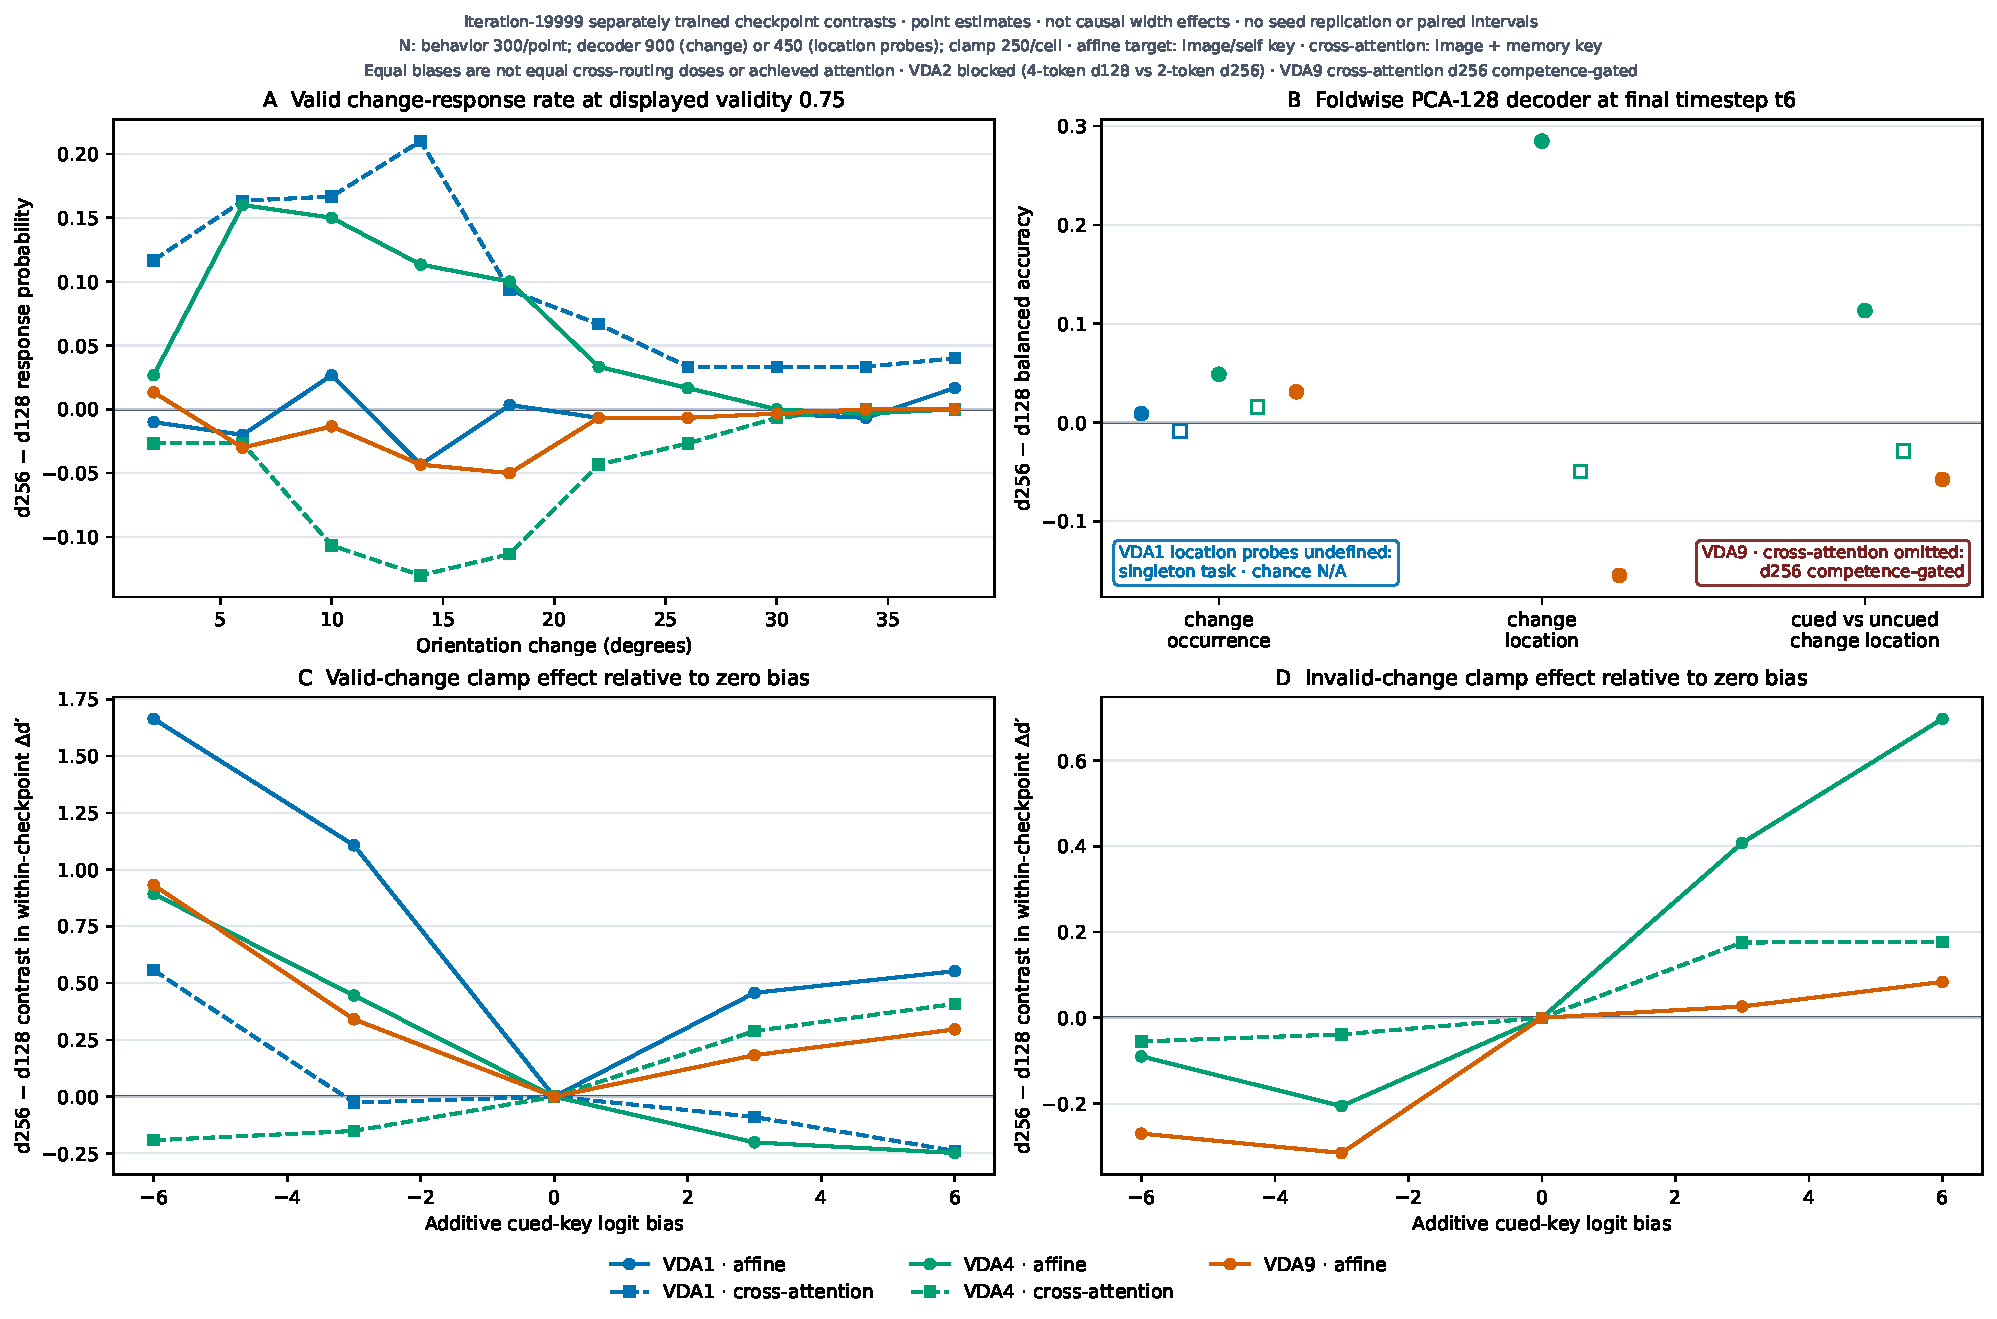
\includegraphics[width=0.78\linewidth]{matched_width_summary.pdf}
\caption{Matched-width negative comparison. The absence of a common signed direction is informative and belongs in the notebook, not as a headline positive result.}
\label{fig:ln-width}
\end{figure}

\smallcapslabel{Memory-decay comparison.}
Two VDA4 checkpoints contrast carried-state decay $\lambda=1.00$ and 0.80. The higher-decay checkpoint shows $+0.108$ frame-to-frame attention total variation (95\% CI $+0.104$ to $+0.112$). This is consistent with faster forgetting accompanying more volatile routing, but one separately trained seed per arm cannot isolate decay causally.

\decisionbox{Amber}{The recurrent state contains change and location information, and memory persistence covaries with routing stability. Neither result demonstrates that attention amplified the target code or that the actor used it. That causal representation bridge remains missing.}

\section{Entry LN-07: Omitted, newly located, and bounded evidence}
\entrymeta{\statusmixed}{Class A/B held-out bundles}{Do existing producer bundles alter the manuscript's stated completion or replication status?}{One frozen checkpoint per bundle}

\subsection{Fixed-carrier K=9 cross-attention seed 0}
A complete producer manifest exists in this repository at
\begin{quote}\footnotesize
\path{reports/vda_series/recommended_experiments_20260729/heldout/vda_fixed9_crossattn1_seed0/}
\end{quote}
It uses 300 psychometric, 128 attention, and 250 intervention trials. At the 100\%-displayed, $30^\circ$ anchor, valid response is 0.940, forced-invalid response 0.903, false alarms 0.030, and $d'$ 3.401 versus 3.151. Natural invalid response is 0.876 versus 0.000 when routing is disabled. A true-location dose sweep yields invalid response 0.044, 0.480, 0.876, 0.984, 0.988 at doses 0, .25, .50, .75, 1.

This bundle corrects the blanket statement that VDA9 is missing or blocked. It does not yet enter the central result spine because it is producer bound and the $30^\circ$ anchor is highly saturated. Correct wording is: \emph{a K=9 producer-bound evaluation exists; independent semantic verification and nonsaturated re-evaluation are pending}.

\subsection{VDA16 cross-attention seed 1 competence failure}
A producer-bound held-out seed-1 bundle also exists, but valid response, invalid response, false alarms, and $d'$ are all zero; natural and disabled invalid response are both zero. This is not a null intervention result in a competent observer. It is a model-level competence failure and must remain in the denominator when discussing how reliably the training procedure produces a usable attentional policy.

\subsection{Independently verified VDA16 affine rescue}
The affine seed-0 true-location rescue is independently verified but close to ceiling: target suppression response 0.7467, natural 0.9800, boost 0.9933, with boost-minus-suppress $d'$ of $+2.2255$. Wrong-location response changes 0.990 to 0.860 and neutral 0.980 to 0.947 over suppression-to-boost. This supports routing dependence in another family, but ceiling compresses the boost and it does not independently verify the cross-attention producer bundle.

\decisionbox{Amber}{The evidence ledger must include a promising but unverified K=9 result, a collapsed VDA16 seed-1 competence failure, and a verified but ceiling-limited affine rescue. Selective reporting only of competent positive checkpoints would overstate generality.}

\section{Entry LN-08: Fixed-100-carrier visual-by-memory stream factorial}
\entrymeta{\statuspending}{Class D training integrity only}{Do effective visual and memory stream counts independently affect binding, routing, representation, and behavior?}{Twelve registered training cells; no held-out scientific unit yet}

\smallcapslabel{Frozen design.}
VDA4 on a fixed 100-token $10\times10$ carrier, cross-attention, effective visual streams $V\in\{4,100\}$, effective memory streams $M\in\{4,100\}$, seeds 0/1/2. All twelve registered runs must execute without result-dependent stopping unless an engineering contract fails. The factorial changes signal rank/binding while leaving all 100 carrier positions in the softmax; it does not isolate eligible-key cardinality.

\smallcapslabel{Training-integrity snapshot.}
Four cells passed terminal training-integrity validation before a simultaneous pod interruption. Three active cells are nonterminal and invalid for conclusions; five registered cells had not yet started. No held-out behavior, attention, representation, or causal bundle from this factorial is admitted.

\begin{table}[H]
\centering\small
\begin{tabularx}{\linewidth}{@{}L{0.09\linewidth}L{0.16\linewidth}L{0.24\linewidth}Y@{}}
\toprule
Seed & Cell & Status & Evidence boundary\\
\midrule
0 & V4/M4 & terminal training integrity & Not held-out scientific evidence\\
0 & V4/M100 & terminal training integrity & Not held-out scientific evidence\\
0 & V100/M4 & interrupted at least through iter 11,973 & Preserve partial; do not resume without complete stochastic/replay state\\
0 & V100/M100 & not yet run & Registered, pending\\
1 & V4/M4 & terminal training integrity & Not held-out scientific evidence\\
1 & V4/M100 & interrupted at least through iter 18,496 & Preserve partial; otherwise rerun fresh in a unique directory\\
1 & V100/M4, V100/M100 & not yet run & Registered, pending\\
2 & V4/M4 & terminal training integrity & Not held-out scientific evidence\\
2 & V4/M100 & interrupted at least through iter 18,507 & Preserve partial; otherwise rerun fresh in a unique directory\\
2 & V100/M4, V100/M100 & not yet run & Registered, pending\\
\bottomrule
\end{tabularx}
\caption{Stream-factorial production status. Completion of training is deliberately separated from completion of the scientific experiment.}
\end{table}

The interrupted hardware is a non-manipulated covariate: seed 0 ran on Ampere RTX3090 while seeds 1/2 ran on Blackwell RTX5080. The workflow record last marked all retained production pods EXITED with runtime absent; this document rewrite neither restarted nor deleted any pod.

\warningbox{Partial directories must never be overwritten. Interrupted cells may be resumed only if model, optimizer, scheduler, RNG, curriculum, environment, and prioritized-replay state are proven fully restorable. Otherwise preserve the partial directory and rerun the registered cell fresh and uninterrupted in a unique replacement directory.}

\decisionbox{Navy}{The entire $V\times M$ factorial is currently engineering/provenance evidence only. Four terminal training cells do not support a scientific statement about visual streams, memory streams, attention, binding, behavior, or scaling.}

\clearpage
\section{Entry LN-09: Proposed decisive coherence-chain experiment}
\entrymeta{\statuspending}{Preregistered future mechanism test}{Does attention causally improve the propagation and decision readout of target information?}{Independent competent training seed; disjoint CRN trial bank}

\smallcapslabel{Core design.}
For competent fixed-carrier $K\in\{4,9,16\}$ checkpoints, use disjoint calibration and evaluation banks. Calibrate change magnitude before the causal experiment to avoid floor and ceiling, then lock it. Apply mass- or entropy-matched interventions at cue, change, and post-change frames, independently targeting the true change, cued-wrong, neutral, uniform, and shuffled controls. Intervene separately on current-image keys, previous-hidden-state keys, and both sources.

On every held-out trial, record:
\begin{itemize}
\item source-separated current-image-key and previous-hidden-state-key routing, including query-region by key-region structure;
\item every spatial memory slot, the full memory vector, and target-versus-distractor representation margins;
\item first actor-layer state, action logits, and change-evidence margin;
\item response, false alarm, $d'$, criterion, and logical response frame.
\end{itemize}

\smallcapslabel{Required coherent signature.}
True-target boost at change time should increase target routing, target-code separability, actor evidence, and $d'$; suppression should reverse all four. Cued-wrong and neutral controls should not reproduce the rescue. Cue-time perturbation should be distinguished from change-time perturbation. A preregistered multilevel mediation analysis should test intervention $\rightarrow$ routing $\rightarrow$ representation $\rightarrow$ actor evidence $\rightarrow$ behavior.

\smallcapslabel{Falsifier.}
The strong theory is weakened if attention changes response without increasing target representation or actor evidence; if a neutral/norm-matched redistribution produces equal rescue; if only frame-6 variables mediate the effect; or if competent seeds do not reproduce the full chain.

\decisionbox{Navy}{This is the missing centerpiece. It tests the proposed function of attention rather than relying on sharp maps or a behavioral effect alone.}

\section{Entry LN-10: Proposed clean distractor-cardinality experiment}
\entrymeta{\statuspending}{Preregistered future scaling test}{Does the number of independently varying distractor keys increase attentional need at fixed object set size?}{Independent seed within a parameter-matched fixed carrier}

Use a constant 100-token carrier, fixed parameters, readout, target information, cue semantics, training budget, and four active items. Vary only the number of independently eligible visual keys—4, 16, or 100—through a fixed mask or controlled equal-energy distractor generator. Broadcasting four signals over 100 repeated keys is a signal-rank manipulation, not a competitor-count manipulation, and cannot serve as the primary test.

Primary preregistered interactions are:
\begin{itemize}
\item eligible-key count $\times$ cue validity on $d'$ and psychometric threshold;
\item eligible-key count $\times$ intervention location on $d'$;
\item eligible-key count $\times$ intervention on target-representation margin;
\item eligible-key count $\times$ intervention on actor-logit margin.
\end{itemize}

Use at least five independent seeds per cell; eight to ten are preferable for a theory-level population claim. Preserve common random numbers within checkpoint, but base population inference on the training seeds. The simple distractor-cardinality hypothesis is directly disconfirmed if these interactions are absent with competent models, nonsaturated evaluation, adequate precision, and fixed parameters.

\decisionbox{Navy}{The native $2\times2/4\times4/10\times10$ battery cannot answer this isolated question. A constant-carrier eligible-key manipulation must be run as a new experiment, not recovered by reinterpreting the old one.}

\section{Entry LN-11: Proposed fixed-carrier active-item series}
\entrymeta{\statuspending}{Preregistered future scaling test}{Does active-object competition, independent of geometry, enlarge cueing and target-specific causal effects?}{Independent seed on a shared carrier and evaluator}

Train $K=4,9,16$ under one carrier, parameterization, cue semantics, training protocol, calibration rule, and evaluation bank. Estimate cue-validity $\times K$ effects on threshold, $d'$, criterion, response frame, source-separated routing, target-code margin, actor evidence, and spatially specific causal rescue. Use at least five seeds per cell and report competence-failure frequency rather than conditioning it away. If budget permits, cross $K$ with eligible-key cardinality to separate object competition from background-patch competition.

The existing cross-attention response gaps 0.27/0.32/0.44 and affine gaps 0.19/0.38/0.32 remain motivation only. A flat or reversed multi-seed $K$ interaction—especially across both routing families—would falsify a general monotonic set-size law.

\decisionbox{Navy}{No current experiment isolates active-item set size from geometry and lineage. The population-level set-size claim remains open.}

\section{Entry LN-12: Replication, calibration, and inference policy}
\entrymeta{\statuspending}{Prospective analysis protocol}{What prevents a fixed-checkpoint effect from being mistaken for a general mechanism?}{Independent training seed}

\begin{enumerate}
\item \textbf{Separate competence from causal success.} Freeze a held-out competence gate before intervention results are inspected. Report all trained seeds and the competence success rate. Analyze intervention effects both unconditionally and, if justified, conditional on the preregistered competence gate.
\item \textbf{Calibrate without peeking.} Use a disjoint calibration bank to choose nonsaturated change magnitudes and intervention doses. Freeze them before the evaluation bank.
\item \textbf{Use common random numbers correctly.} CRN reduces within-checkpoint trial noise. It does not create independent model replicates.
\item \textbf{Make the seed the inferential unit.} Trial bootstrap intervals describe a frozen checkpoint. Population claims require seed-level contrasts or hierarchical models over independent training runs.
\item \textbf{Predeclare the frame and estimand.} Frame 5 is the decision-relevant primary event frame; frame 6 is secondary. Equal-area regional mass is primary across grids; maximum-patch statistics are secondary and require an $N$-matched null.
\item \textbf{Require semantic verification.} Recompute scientific metrics independently from source arrays, not only hashes. Preserve visual and memory source identity, trial IDs, query/key regions, logits, and representations.
\item \textbf{No result-dependent stopping.} All registered cells run to their engineering contract unless that contract fails. Negative, collapsed, interrupted, and saturated cells remain visible.
\end{enumerate}

\decisionbox{Navy}{A scientific theory is supported by replicated interactions and converging links, not by the number of trials, plots, checkpoint files, or training rows.}

\clearpage
\section{Entry LN-13: Registered VDA4 mnemonic-interference pilot}
\entrymeta{\statuspending}{Frozen paired-pilot protocol; no scientific result}{Does independent Gaussian corruption of recurrent cell content increase cueing and the causal value of selective routing?}{One paired seed-0 training contrast; four crossed held-out evaluation cells}

\smallcapslabel{Hypothesis and lineage.}
The narrow prediction is that destructive interference makes task-relevant signals harder to preserve against competitors, thereby increasing the functional value of selective routing. The pilot uses native VDA4 with four active items, four $2\times2$ current-image tokens and four recurrent locations, cross-attention, $d_{\mathrm{mem}}=128$, memory decay 1, seed 0, and 20,000 fresh training iterations. The registered manipulation is $\sigma\in\{0,0.5\}$ in the xLSTM carried cell content,
\begin{equation}
C_t \leftarrow C_t^{\mathrm{clean}} + \sigma\,(N_t^{\mathrm{norm}}+10^{-8})\odot\epsilon_t,
\qquad \epsilon_t\sim\mathcal{N}(0,I),
\end{equation}
with an independent draw for every batch element, native memory slot, memory coordinate, and injected update. Here $N_t^{\mathrm{norm}}$ is the xLSTM normalizer state, not the number of image patches. The $0.5$ dose is a newly registered VDA dose. It is not an exact repeat of the earlier normalized LayerNorm-cell run at $\sigma=0.05$, which produced an always-declare observer, and it must not be conflated with Luo--Maunsell configurations in which 0.5 denoted memory decay and/or sensory orientation jitter.

\smallcapslabel{Frozen training comparison.}
The two training runs share the same named trainable initialization, execute sequentially on the same physical GPU and software fingerprint, and cannot be stopped according to intermediate accuracy, curriculum, attention, or effect direction. They do not share an asserted on-policy training trajectory: injected noise may change actions and episode lengths, after which environment random-number consumption can diverge. Common random numbers are reserved for the disjoint held-out trial banks. The current trainer is explicitly asymmetric: rollout and optimized student/replay passes receive mnemonic noise, while target actor/critic and JEPA-teacher passes remain noise-off. A later all-networks-noisy experiment would be a different protocol.

\begin{table}[H]
\centering\small
\begin{tabularx}{0.94\linewidth}{@{}L{0.17\linewidth}L{0.17\linewidth}Y@{}}
\toprule
Training $\sigma$ & Evaluation $\sigma$ & Question answered\\
\midrule
0 & 0 & Deterministic-memory baseline\\
0 & 0.5 & Acute interference in an unadapted checkpoint\\
0.5 & 0 & Persistent learned reorganization when acute test noise is removed\\
0.5 & 0.5 & Matched noisy-training and noisy-evaluation condition\\
\bottomrule
\end{tabularx}
\caption{The complete held-out $2\times2$ factorial separates acute corruption from training-time adaptation. The matched total contrast is train0/eval0 versus train0.5/eval0.5; the adaptation contrast holds evaluation noise at 0.5.}
\end{table}

\smallcapslabel{Evidence chain and failure rule.}
The hypothesis is supported at seed 0 only if three held-out links align: (1) the noisy condition increases the cue-validity effect on psychometric threshold and $d'$ without a criterion-only explanation or floor/ceiling; (2) current-image-key and previous-hidden-state-key routing, displayed in separate maps, becomes more selectively aligned with the cue during t1--t4 and with the true changed location during t5--t6; and (3) graded routing-logit interventions have a larger, orderly, spatially specific behavioral effect at the true-change location than at cued-wrong and neutral-control locations. Validities 0.25, 0.50, and 0.75 define the in-distribution trend. Forced-invalid trials at displayed validity 1 are an expectancy-violation probe and are excluded from that primary slope.

For every source and key, the primary patch score remains the column average $p_s(j)=N_q^{-1}\sum_i A_{ij}$. Current-image-key and previous-hidden-state-key $4\times4$ query-by-key arrays are preserved and reduced separately onto the common physical $2\times2$ grid. The memory-noise manipulation acts on xLSTM cell content $C$; cross-attention later reads keys projected from recurrent hidden output $H$, so these are related but not identical tensors. Because the model is natively $2\times2$, region total and region maximum are identical and cannot be counted as independent corroboration. A sharper map without sensitivity and spatially specific causal dependence is descriptive redistribution, not evidence that attention increased signal coherence.

\smallcapslabel{Engineering status on 3 August 2026.}
The frozen package is at \path{RViT_plus_paper_jepa_grid9/experiments/vda4_memory_noise/grid2x2_crossattn1_pilot_v1/}. Its frozen identities are:
\begin{description}[leftmargin=1.35in,labelwidth=1.18in,itemsep=1pt,topsep=3pt]
  \item[Design SHA-256] \texttt{1ae15e32\allowbreak b3568750\allowbreak 1554463a\allowbreak 714074b6\allowbreak 774e70ae\allowbreak d524780f\allowbreak f14a733d\allowbreak 832ec97b}
  \item[Config SHA-256] \texttt{01971fd7\allowbreak 31e030ed\allowbreak 377f0c7d\allowbreak b1164f0c\allowbreak f8c01285\allowbreak fbb57e7e\allowbreak da7381ae\allowbreak d2414eb7}
\end{description}
Seventy-nine relevant local tests and all four registered canary/production preflights pass. Those checks establish engineering integrity only. No canary, 20,000-iteration training pair, terminal artifact, or held-out behavioral/mechanistic evaluation has yet been run.

\decisionbox{Navy}{This is the immediate directional pilot for the interference hypothesis, not evidence for it. A coherent seed-0 result would justify a separately frozen multi-seed replication; a competent null result would constrain this dose and trainer, not every possible noise level or recurrent-noise algorithm.}

\part*{Part III --- Measurement dictionary, diagnostic plates, and provenance}
\addcontentsline{toc}{section}{Part III --- Measurement dictionary, diagnostic plates, and provenance}

\section{Exact attention-map reduction and comparison rules}
This section resolves the ambiguity that motivated the rewrite. Let $A_{bij}$ be the registered query-to-key routing matrix for trial $b$ at a named frame, after the evaluator's registered head reduction. Index $i$ runs over $N_q=N$ current-image queries. In cross-attention, keys 1 through $N$ are projected from current-image tokens $X_t$, and keys $N+1$ through $2N$ are projected from the previous recurrent hidden output $H_{t-1}$. One softmax normalizes across all $2N$ keys.

\subsection{Split the sources before any reduction}
For each spatial key $j$, first average down its column across all queries, keeping the two key sources separate:
\begin{equation}
p^X_{bj}=\frac{1}{N_q}\sum_{i=1}^{N_q}A_{bi,j},
\qquad
p^H_{bj}=\frac{1}{N_q}\sum_{i=1}^{N_q}A_{bi,N+j}.
\end{equation}
The source shares are
\begin{equation}
w^X_b=\sum_jp^X_{bj},\qquad w^H_b=\sum_jp^H_{bj},\qquad w^X_b+w^H_b=1.
\end{equation}
This is the literal ``sum down the patch's column and divide by the number of patches'' operation: the divisor is the number of query patches. The $p^X$ and $p^H$ vectors are then mapped separately. They are never added to create an attention map.

\subsection{Map every native grid to the same physical four regions}
Partition the image into a fixed physical $2\times2$ grid with quadrants $Q_r$, regardless of native discretization. A $2\times2$ model contributes one native patch per quadrant, a $4\times4$ model four, and a $10\times10$ model 25. The primary equal-area regional mass and the requested maximum-patch regional score are:
\begin{equation}
T^s_{br}=\sum_{j\in Q_r}p^s_{bj},
\qquad
P^s_{br}=\max_{j\in Q_r}p^s_{bj},
\qquad s\in\{X,H\}.
\end{equation}
$T_r$ asks how much routing reaches the same physical region. $P_r$ asks whether any one native patch inside that region receives a strong column-averaged weight. These are not interchangeable.

\subsection{Report raw and normalized quantities together}
Under globally uniform cross-attention, one source's raw quadrant total is $1/8$ and one key's raw mass is $1/(2N)$. Therefore $2NP^s_{br}$ has a uniform baseline of one. Because a maximum over more patches has a larger extreme-value opportunity even after simple uniform scaling, every peak comparison also requires an $N$-matched null generated under the registered constraint structure.

Source-conditional target mass $T^s_{br}/w^s_b$ asks where a source routes \emph{given} that the joint softmax used that source. It must be displayed beside $w^s_b$; otherwise a tiny source can look artificially decisive after renormalization. Peak-quadrant share and within-quadrant focality are useful secondary descriptors, not replacements for raw source mass. For affine feedback, this two-source decomposition does not exist: $H_{t-1}$ generates scale and shift for $X_t$, after which self-attention routes only among modulated current-image keys.

\begin{table}[H]
\centering\small
\begin{tabularx}{\linewidth}{@{}L{0.22\linewidth}L{0.25\linewidth}Y@{}}
\toprule
\smallcapslabel{Measure} & \smallcapslabel{Question answered} & \smallcapslabel{Required caveat}\\
\midrule
Source share $w_s$ & How much of the joint softmax went to visual versus memory keys? & Says nothing about localization within source\\
Equal-area total $T^s_r$ & How much raw routing reached the same physical quadrant? & Primary cross-grid spatial comparison\\
Maximum patch $P^s_r$ & What is the strongest column-averaged native patch inside the region? & Secondary; grid-dependent extreme-value null\\
$2NP^s_r$ & How strong is the maximum relative to a globally uniform cross key? & Uniform correction does not remove heterogeneous-max opportunity\\
Conditional total $T^s_r/w_s$ & Where did a source route, conditional on selecting that source? & Must be shown with source share\\
Target-minus-distractor & Does routing discriminate the task-relevant location? & Predeclare target, comparison set, and event frame\\
Paired $V+M$ location & How much total routing reaches co-located visual and memory keys? & Secondary only; not either source map or either source maximum\\
Full query-region $\times$ key-region matrix & Which query regions route to which key regions? & Preserve in machine-readable arrays even when a spatial summary is plotted\\
\bottomrule
\end{tabularx}
\caption{Attention measures are named by the question they answer. The manuscript must never call all of them an undifferentiated ``attention score.''}
\end{table}

\warningbox{The distinct statistic $\max_i A_{bij}$ is the strongest single query-to-key link. It is not the requested $\max_j\operatorname{mean}_i A_{bij}$ maximum-patch regional score and must not be substituted for it.}

\section{Behavioral and statistical estimands}
The four-parameter psychometric fit is
\begin{equation}
p(x)=\gamma+\frac{1-\gamma-\lambda}{1+\exp[-(x-\alpha)/\beta]},
\end{equation}
where $\alpha$ is threshold, $\beta$ slope, $\gamma$ guess rate, and $\lambda$ lapse rate. Threshold cost and valid-minus-invalid response-gap AUC compare whole curves rather than one easy endpoint.

Signal detection uses
\begin{equation}
d'=\Phi^{-1}(H)-\Phi^{-1}(F),\qquad
c=-\tfrac12[\Phi^{-1}(H)+\Phi^{-1}(F)],
\end{equation}
with the registered finite-count correction applied by the evaluator. A response-rate increase supports coherence only when $d'$, threshold, latency, utility, or representation also improve; a criterion change alone is not enough.

Conditional mean response frame summarizes only trials with a qualifying declaration and therefore must be read beside response probability. It cannot distinguish a fast observer from one that responds on very few easy trials unless both quantities are shown.

Trial bootstrap and Wilson intervals quantify finite held-out-trial variation for one fixed checkpoint. Paired CRN intervals quantify within-checkpoint contrasts. Neither estimates variation over training seeds. Seedwise uncertainty and competence frequency are mandatory for a population claim.

\section{Selected diagnostic plates}
These plates retain scientifically useful diagnostics without interrupting the core causal sequence.

\subsection{VDA16 psychometric overlays}
\begin{figure}[H]
\centering
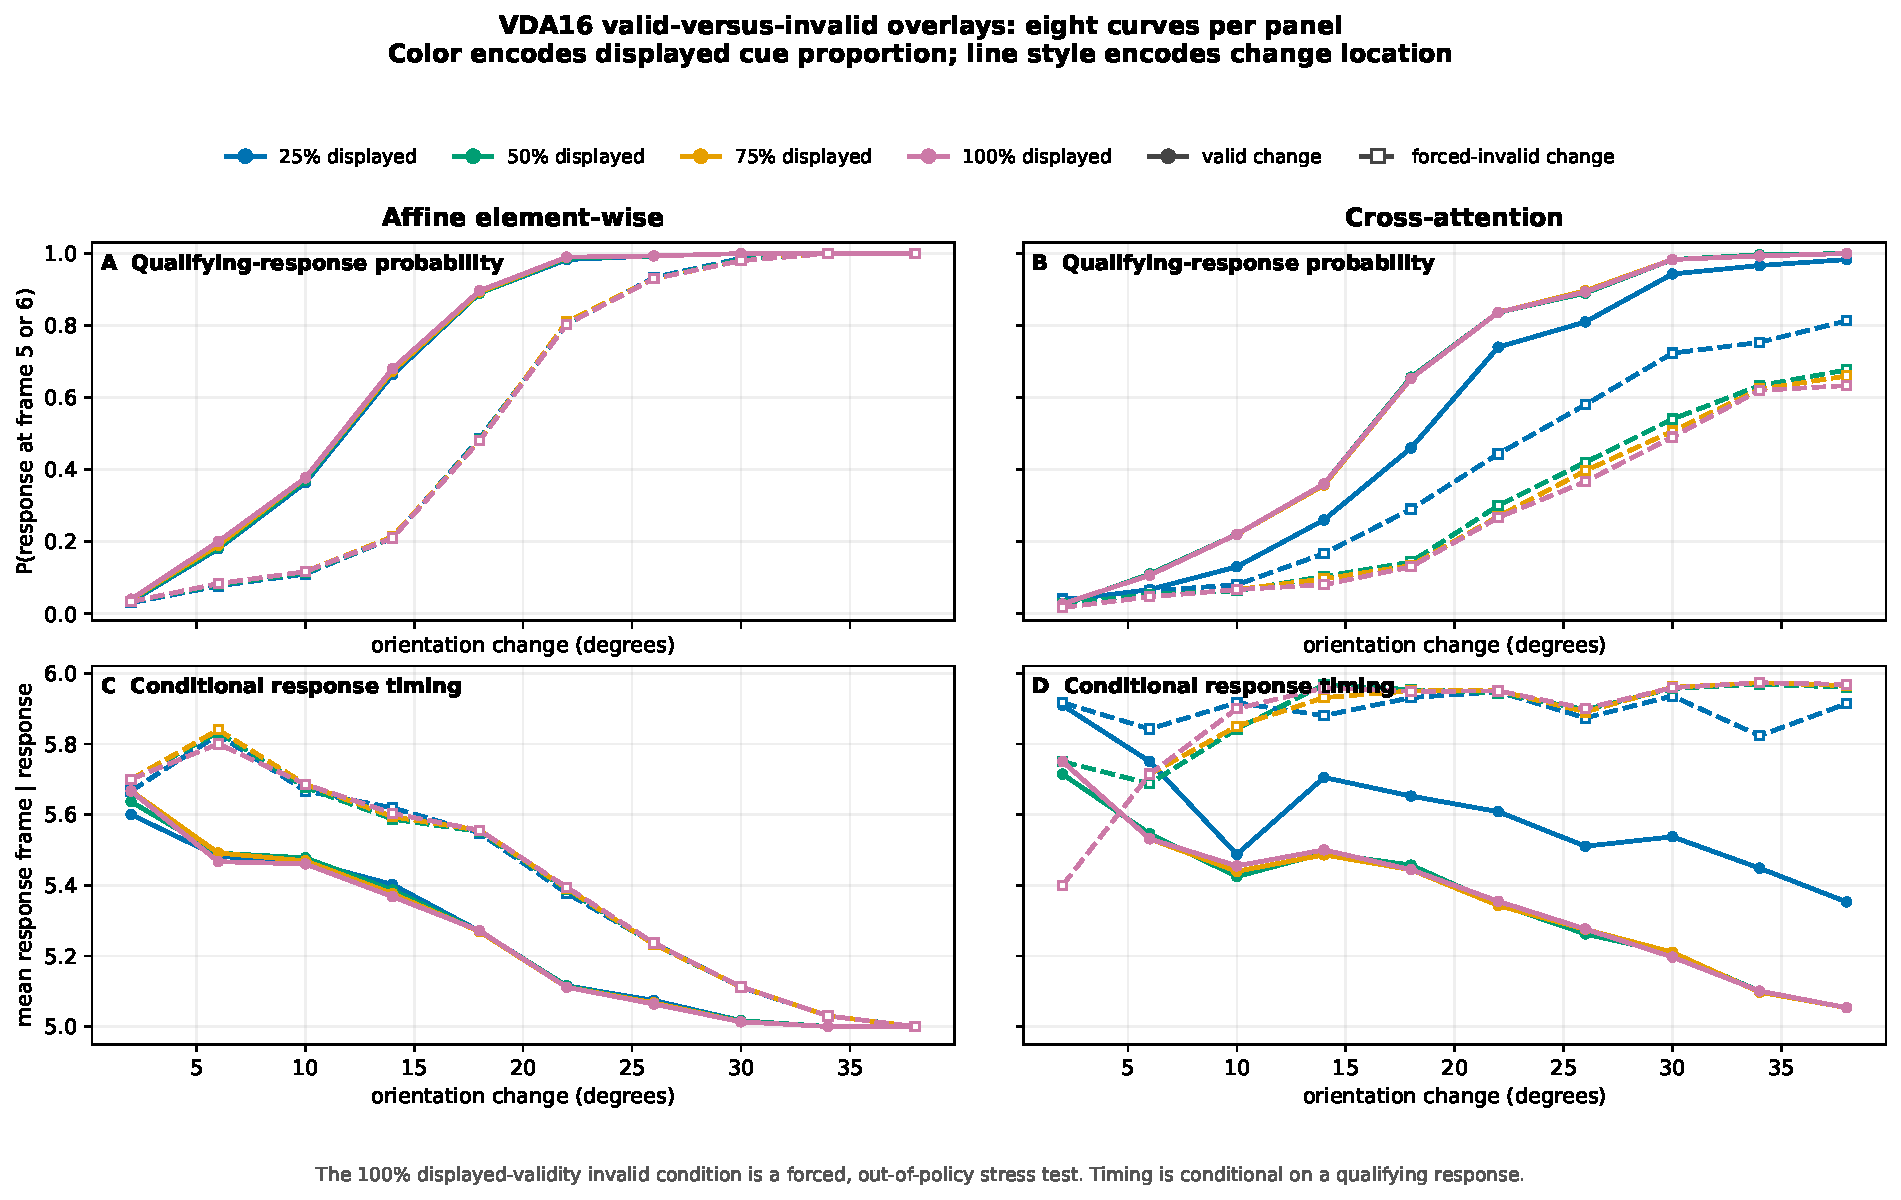
\includegraphics[width=0.76\linewidth]{vda16_valid_invalid_eight_curve_overlay.pdf}
\caption{Cross-attention separates valid and forced-invalid curves across displayed cue proportions; affine separates mainly in the 100\%-displayed out-of-policy stress test. The routing-family contrast is descriptive because checkpoint competence and training history differ.}
\end{figure}

\subsection{Frame-specific attention diagnostics}
\begin{figure}[H]
\centering

\includegraphics[width=0.78\linewidth]{attention_framewise_comparison_seed0.pdf}
\caption{Frame 5 and frame 6 are separate estimands. Cross-attention panels shown here are secondary paired-location totals; source-separated maps follow.}
\end{figure}

\subsection{Two-seed endpoint directions}
\begin{figure}[H]
\centering

\includegraphics[width=0.76\linewidth]{vda4_spatial_scaling_endpoint_replication_summary.pdf}
\caption{Cross-attention endpoints at seeds 0 and 1. Behavioral directions disagree and the seed-1 100-token intervention is saturated. Two seeds support directional description, not population inference.}
\end{figure}

\begin{figure}[H]
\centering

\includegraphics[width=0.74\linewidth]{attention_endpoint_replication_multimetric.pdf}
\caption{The endpoint conclusion changes with the named frame-5 estimator. Trial-bootstrap intervals remain within-checkpoint intervals.}
\end{figure}

\subsection{Native source-separated time courses}
The following plates deliberately repeat one display convention across grids: rows are visual-valid, visual-invalid, memory-valid, and memory-invalid; columns are t0--t6; one raw scale is used; source share is printed; cue and true change are separately marked.

\begin{figure}[H]
\centering

\includegraphics[width=0.96\linewidth]{attention_crossattn_source_timecourse_grid2x2_seed0.pdf}
\caption{$2\times2$ cross-attention source time course.}
\end{figure}

\begin{figure}[H]
\centering

\includegraphics[width=0.96\linewidth]{attention_crossattn_source_timecourse_grid4x4_seed0.pdf}
\caption{$4\times4$ cross-attention source time course, with the same physical quadrant boundaries.}
\end{figure}

\begin{figure}[H]
\centering

\includegraphics[width=0.96\linewidth]{attention_crossattn_source_timecourse_grid10x10_seed0.pdf}
\caption{$10\times10$ cross-attention source time course at native resolution. The grid is not upsampled and the sources are not collapsed.}
\end{figure}

\section{Production freeze and interruption record}
The frozen stream-factorial source bundle is \path{reports/vda_series/stream_factorial_production_20260730/rvit_stream_factorial_source_20260730T161426Z.tar.gz}, SHA-256
\begin{quote}\ttfamily\small d943ca758ed15cbea98d82fd8da02f3114c4bb9958845e31f2e125d0a61c17f6\end{quote}

\begin{table}[H]
\centering\scriptsize
\begin{tabularx}{\linewidth}{@{}L{0.18\linewidth}Y@{}}
\toprule
Frozen object & SHA-256\\
\midrule
Training script & \texttt{713d337781f432d9419189bb66cdd5c7abd2e3986e072c8be94216700814421c}\\
Configuration & \texttt{f5b62e32e40e2d8c5ee97ae71e2c520737fbf431ff4b64f82b58c718b23eb6aa}\\
Design & \texttt{8a82292d725eb7519c4c394a0ddfe9037aac2a60fa02476e1ce241e76b9daf76}\\
Preflight & \texttt{6d92391c7545c0ba558193a0b9aa28b0cc24bca8234238b0ccb78d6d7f4269be}\\
Production launcher & \texttt{bc0b1b7c02c8ad321dcb8af510f7b40b1b394d56eff3f7e70928ba2bc07182ff}\\
Queue & \texttt{a8e960120b46982985a8b2d049008483a2428fc9fc9a9f14ef89806f93e2c1b2}\\
\bottomrule
\end{tabularx}
\caption{Frozen production inputs. Hash integrity establishes provenance, not a scientific result.}
\end{table}

The four terminal training-integrity pairs are preserved below. ``Final'' and ``latest'' are separately hashed because semantic equality, not byte equality, is the terminal contract.

\begingroup\scriptsize
\begin{longtable}{@{}L{0.16\linewidth}L{0.36\linewidth}L{0.36\linewidth}@{}}
\toprule
Cell & Final SHA-256 & Latest SHA-256\\
\midrule\endhead
seed0 V4/M4 & \texttt{e95253fea3fb485d3d8cda61f3af685\allowbreak c026b2b57e42e358de211cc4dd49af30f} & \texttt{102ca2fecf10580f361a596ada744d64\allowbreak cee913269bcd661cad19fea6f506a2fe}\\
seed0 V4/M100 & \texttt{bcfedeb5600e9c0ef8c4d5ee2a98bd2\allowbreak f1e956722f6d5b5fac71eb23017ac9296} & \texttt{afa58603d3ea4400148c0a611a408b74\allowbreak 5e27d50cce91af05d98cf4d715146dc3}\\
seed1 V4/M4 & \texttt{194bad7230faf8d16f088ecd599917866\allowbreak 6ac815e953282ca57ae4768db03366a} & \texttt{011cb753effcc07995e2bb59e1b4de0c\allowbreak cdd89faa9e20e6e4d6235578c1b7c5b6}\\
seed2 V4/M4 & \texttt{afe9ef868c8c924283a7f9526d8a3a8\allowbreak f8fd325cb0a86d0aba00aa6422f93fdee} & \texttt{5fece31503f106cda30ad7af6499a597\allowbreak 2c0305d4198ecd17393e47315449e48c}\\
\bottomrule
\end{longtable}
\endgroup

On 31 July 2026 at 00:31 UTC, three production pods simultaneously changed from healthy RUNNING to EXITED with runtime absent. The cause was not established. Their persistent workspaces and two earlier failed RTX3090 host-diagnostic pods were retained. No pod may be deleted; no retained production pod may be restarted without explicit billing/capacity authorization. This interruption is part of the laboratory record and not a scientific manipulation.

\section{Artifact register}
The full 952-cell panel disposition matrix, raw path inventory, and historical contact sheets remain in the preserved original manuscript and machine-readable artifacts. This notebook keeps a shorter human-readable index.

\begin{longtable}{@{}L{0.24\linewidth}L{0.48\linewidth}L{0.20\linewidth}@{}}
\toprule
Artifact & Path & Role\\
\midrule\endhead
Preserved original PDF & \path{reports/vda_series/manuscript/VDA_Set_Size.pdf} & Complete prior narrative and inventory\\
Preserved original source & \path{reports/vda_series/manuscript/main.tex} & Source of the 41-page manuscript\\
Herman--Morgan reference & \path{reports/vda_series/source_material/mah/2502.10955v1.pdf} & Narrative and experimental benchmark\\
Task figures & \path{reports/vda_series/figures/task/} & Deterministic specifications\\
Architecture figures & \path{reports/vda_series/figures/architecture/} & Source-derived diagrams\\
First-wave products & \path{reports/vda_series/figures/first_wave/} & VDA4/VDA9 behavior and source maps\\
VDA16 figures & \path{reports/vda_series/figures/vda16/} & Behavior, attention, SDT, and interventions\\
Spatial scaling & \path{RViT_plus_paper_jepa_grid9/reports/vda_series/spatial_scaling_evaluation_production_20260727/} & Six-cell seed-0 held-out battery\\
Endpoint replication & \path{RViT_plus_paper_jepa_grid9/reports/vda_series/spatial_scaling_evaluation_production_20260727/endpoint_replication_s01/} & Two grids by two cross-attention seeds\\
Source refresh & \path{RViT_plus_paper_jepa_grid9/reports/vda_series/spatial_scaling_crossattn_source_attention_20260803/} & Visual/memory source preservation\\
Attention-measure bundle & \path{RViT_plus_paper_jepa_grid9/reports/vda_series/spatial_scaling_attention_measures_20260803_source_separated_v6/} & Common-grid metrics and vector figures\\
K=9 producer bundle & \path{RViT_plus_paper_jepa_grid9/reports/vda_series/recommended_experiments_20260729/heldout/vda_fixed9_crossattn1_seed0/} & Pending independent semantic verification\\
Stream-factorial tracker & \path{reports/vda_series/stream_factorial_production_20260730/RUNPOD_PRODUCTION_LAUNCH_MANIFEST.json} & Training/provenance status only\\
Memory-interference pilot & \path{RViT_plus_paper_jepa_grid9/experiments/vda4_memory_noise/grid2x2_crossattn1_pilot_v1/} & Frozen paired-pilot design, launch contracts, evaluator, and tests; unrun\\
\bottomrule
\end{longtable}

\section{Final scientific synthesis}
The readable version of the VDA story is not ``attention rises with more tokens.'' It is:

\begin{enumerate}
\item The models can show cue-dependent detection, and at VDA16 the gap includes sensitivity as well as criterion.
\item Current-image-key and previous-hidden-state-key routing exhibit distinct cue- and event-aligned dynamics; collapsing them erases source information.
\item At selected cross-attention checkpoints, routing at the true change location is behaviorally causal and spatially specific.
\item Cross-attention's cueing effect grows descriptively with active-item set size, but affine does not show the same monotonic sequence and the comparison is confounded.
\item A fixed-four-item native-grid test does not support a universal monotonic discretization law. Source, metric, frame, family, and seed matter.
\item The proposed theory remains open because the end-to-end causal chain from routing through target representation and actor evidence to sensitivity-corrected behavior has not yet been demonstrated across independent seeds.
\item A frozen native-VDA4 memory-interference pilot now tests whether independent recurrent-state corruption increases cue dependence, source-resolved target allocation, and spatially specific causal reliance. It is registered and preflighted but unrun.
\end{enumerate}

The current evidence is therefore meaningful but narrower than the theory. It supports a checkpoint-local claim that spatial routing can govern whether a target is detected. It motivates, but does not yet prove, the stronger claim that attention's general function is to increase signal coherence under competition. The registered memory-interference pilot is a useful next directional test because it deliberately raises mnemonic competition and requires behavior, source-resolved allocation, and causal use to move together. The decisive theory-level advance remains a preregistered, independently verified, multi-seed experiment in which target routing, target representation, actor evidence, and behavior are measured and causally linked on the same nonsaturated held-out trials.

\begin{thebibliography}{9}
\small
\bibitem{mah2025} J.~Morgan, B.~Albanna, and J.~P.~Herman. A recurrent vision transformer shows signatures of primate visual attention. \emph{arXiv:2502.10955v1}, 2025.
\bibitem{carrasco2011} M.~Carrasco. Visual attention: the past 25 years. \emph{Vision Research}, 2011.
\bibitem{luo2018} T.~Z.~Luo and J.~H.~R.~Maunsell. Attentional changes in either criterion or sensitivity are associated with robust modulations in lateral prefrontal cortex. \emph{Neuron}, 2018.
\bibitem{moore2003} T.~Moore and K.~M.~Armstrong. Selective gating of visual signals by microstimulation of frontal cortex. \emph{Nature}, 2003.
\bibitem{cavanaugh2004} J.~Cavanaugh and R.~H.~Wurtz. Subcortical modulation of attention counters change blindness. \emph{Journal of Neuroscience}, 2004.
\bibitem{luck1997} S.~J.~Luck and E.~K.~Vogel. The capacity of visual working memory for features and conjunctions. \emph{Nature}, 1997.
\bibitem{awh2001} E.~Awh and J.~Jonides. Overlapping mechanisms of attention and spatial working memory. \emph{Trends in Cognitive Sciences}, 2001.
\bibitem{panichello2021} M.~F.~Panichello and T.~J.~Buschman. Shared mechanisms underlie the control of working memory and attention. \emph{Nature}, 2021.
\end{thebibliography}

\end{document}
